%%%%%%%%%%%%%%%%%%%%%%%%%%%%%%%%%%%%%%%%%%%%%%%%%%%%%%%%%%%%%%%%%%%%%
%%                                                                 %%
%% Please do not use \input{...} to include other tex files.       %%
%% Submit your LaTeX manuscript as one .tex document.              %%
%%                                                                 %%
%% All additional figures and files should be attached             %%
%% separately and not embedded in the \TeX\ document itself.       %%
%%                                                                 %%
%%%%%%%%%%%%%%%%%%%%%%%%%%%%%%%%%%%%%%%%%%%%%%%%%%%%%%%%%%%%%%%%%%%%%

%%\documentclass[referee,sn-basic]{sn-jnl}% referee option is meant for double line spacing

%%=======================================================%%
%% to print line numbers in the margin use lineno option %%
%%=======================================================%%

%%\documentclass[lineno,sn-basic]{sn-jnl}% Basic Springer Nature Reference Style/Chemistry Reference Style

%%======================================================%%
%% to compile with pdflatex/xelatex use pdflatex option %%
%%======================================================%%

%%\documentclass[pdflatex,sn-basic]{sn-jnl}% Basic Springer Nature Reference Style/Chemistry Reference Style

%%\documentclass[sn-basic]{sn-jnl}% Basic Springer Nature Reference Style/Chemistry Reference Style
\documentclass[pdflatex,sn-mathphys]{sn-jnl}% Math and Physical Sciences Reference Style
%%\documentclass[sn-aps]{sn-jnl}% American Physical Society (APS) Reference Style
%%\documentclass[sn-vancouver]{sn-jnl}% Vancouver Reference Style
%%\documentclass[sn-apa]{sn-jnl}% APA Reference Style
%%\documentclass[sn-chicago]{sn-jnl}% Chicago-based Humanities Reference Style
%%\documentclass[sn-standardnature]{sn-jnl}% Standard Nature Portfolio Reference Style
%%\documentclass[default]{sn-jnl}% Default
%%\documentclass[default,iicol]{sn-jnl}% Default with double column layout

%%%% Standard Packages
%%<additional latex packages if required can be included here>
%%%%

%%%%%=============================================================================%%%%
%%%%  Remarks: This template is provided to aid authors with the preparation
%%%%  of original research articles intended for submission to journals published 
%%%%  by Springer Nature. The guidance has been prepared in partnership with 
%%%%  production teams to conform to Springer Nature technical requirements. 
%%%%  Editorial and presentation requirements differ among journal portfolios and 
%%%%  research disciplines. You may find sections in this template are irrelevant 
%%%%  to your work and are empowered to omit any such section if allowed by the 
%%%%  journal you intend to submit to. The submission guidelines and policies 
%%%%  of the journal take precedence. A detailed User Manual is available in the 
%%%%  template package for technical guidance.
%%%%%=============================================================================%%%%
\usepackage{parskip}
\usepackage{caption}
\usepackage{adjustbox}
\usepackage{multirow}
\begin{document}

\title[SREMIC: Spatial Relation Extraction-based Malware Image Classification]{SREMIC: Spatial Relation Extraction-based Malware Image Classification}


\author[1]{\fnm{Inzamamul} \sur{Alam}}\email{inzimunna@gmail.com}
\equalcont{These authors contributed equally to this work.}

\author[1]{\fnm{Nawmi} \sur{Nujhat}}\email{nujhat98@gmail.com}
\equalcont{These authors contributed equally to this work.}

\author*[1]{\fnm{Dr. Md} \sur{Samiullah}}\email{samiullah@du.ac.bd}


\author[1]{\fnm{Dr. Upama} \sur{Kabir}}\email{upama@cse.du.ac.bd}

\affil*[1]{\orgdiv{Department of Computer Sciene and Engineering}, \orgname{University of Dhaka}, \orgaddress{\street{Nilkhet Road}, \city{Dhaka}, \postcode{1000}, \country{Bangladesh}}}


%%==================================%%
%% sample for unstructured abstract %%
%%==================================%%

\abstract{Around 8,00,000 people fall prey to cyberattacks annually~\cite{36}, most often by ``malware''. Malware has the potential to become destructive weapon in Cyber-world. It is a difficult task to manually thwart an assault by a malware. It is crucial to properly categorize malware binaries in order to identify their origins. Furthermore, malware structure discovery through basic feature extraction approaches are time-consuming and challenging. Malware classification was previously solved using naive ML(Machine-Learning) approaches like SVM and XGBoost. Recently, Deep Learning has proved to be impactful in finding malicious patterns. Without DL, analysis of the vast amounts of available data tends to impossible. Existing methods, such as ``Transfer-Learning''~\cite{33}, ``Fusion-Methodology''~\cite{25}, and ``Ensemble-Learning''~\cite{26}, lack the evidence of effectiveness when tested on actual malware binary files. Moreover, Single image-based malware classification, such as, Gibert et al~.~\cite{19} use rudimentary CNN that does not perform well. For the challenges mentioned above, we propose a novel approach  with a  spatial convolutional neural network with sufficient regularization and data augmentation that can identify and classify malware in images effectively and efficiently. Our model is evaluated using datasets like MalImg~\cite{11}, Microfsoft-Big~\cite{10} and \color{blue}Malevis~\cite{39}\color{black}. The proposed method achieves validation score of 99.93\% for MalImg, 99.72\% for Microsoft-Big and \color{blue}99.22\% for Malevis datasets\color{black}. Our method outperforms VGG16, VGG19, ResNet50, EfficientNetB1, and Google's inceptionV3 including State-Of-The-Art (SOTA) techniques.}

%%================================%%
%% Sample for structured abstract %%
%%================================%%

% \abstract{\textbf{Purpose:} The abstract serves both as a general introduction to the topic and as a brief, non-technical summary of the main results and their implications. The abstract must not include subheadings (unless expressly permitted in the journal's Instructions to Authors), equations or citations. As a guide the abstract should not exceed 200 words. Most journals do not set a hard limit however authors are advised to check the author instructions for the journal they are submitting to.
% 
% \textbf{Methods:} The abstract serves both as a general introduction to the topic and as a brief, non-technical summary of the main results and their implications. The abstract must not include subheadings (unless expressly permitted in the journal's Instructions to Authors), equations or citations. As a guide the abstract should not exceed 200 words. Most journals do not set a hard limit however authors are advised to check the author instructions for the journal they are submitting to.
% 
% \textbf{Results:} The abstract serves both as a general introduction to the topic and as a brief, non-technical summary of the main results and their implications. The abstract must not include subheadings (unless expressly permitted in the journal's Instructions to Authors), equations or citations. As a guide the abstract should not exceed 200 words. Most journals do not set a hard limit however authors are advised to check the author instructions for the journal they are submitting to.
% 
% \textbf{Conclusion:} The abstract serves both as a general introduction to the topic and as a brief, non-technical summary of the main results and their implications. The abstract must not include subheadings (unless expressly permitted in the journal's Instructions to Authors), equations or citations. As a guide the abstract should not exceed 200 words. Most journals do not set a hard limit however authors are advised to check the author instructions for the journal they are submitting to.}


%%\pacs[JEL Classification]{D8, H51}

%%\pacs[MSC Classification]{35A01, 65L10, 65L12, 65L20, 65L70}

\keywords{Malware Classification, Deep Learning, Convolutional Neural Network (CNN), Spatial Relation}

\maketitle
\section{Introduction}\label{introduction}



\begin{table}[tbh]
\begin{adjustbox}{width=\textwidth}
\begin{tabular}{|cc|ccccccc|ccccccc|ccccccc|}
\hline
\multicolumn{1}{|c|}{\multirow{2}{*}{\textbf{VID}}}     & \multirow{2}{*}{\textbf{TTO}}    & \multicolumn{7}{c|}{\textbf{Week, t = 1}}                                                                                                                                                                                            & \multicolumn{7}{c|}{\textbf{Week, t = 2}}                                                                                                                                                                                            & \multicolumn{7}{c|}{\textbf{Week, t = 3}} \\                                                                                           
\cline{3-23}
% \hline
\multicolumn{1}{|c|}{}                                  &                                  & \multicolumn{1}{c|}{\textbf{Sat}} & \multicolumn{1}{c|}{\textbf{Sun}} & \multicolumn{1}{c|}{\textbf{Mon}} & \multicolumn{1}{c|}{\textbf{Tue}} & \multicolumn{1}{c|}{\textbf{Wed}} & \multicolumn{1}{c|}{\textbf{Thu}} & \textbf{Fri} & \multicolumn{1}{c|}{\textbf{Sat}} & \multicolumn{1}{c|}{\textbf{Sun}} & \multicolumn{1}{c|}{\textbf{Mon}} & \multicolumn{1}{c|}{\textbf{Tue}} & \multicolumn{1}{c|}{\textbf{Wed}} & \multicolumn{1}{c|}{\textbf{Thu}} & \textbf{Fri} & \multicolumn{1}{c|}{\textbf{Sat}} & \multicolumn{1}{c|}{\textbf{Sun}} & \multicolumn{1}{c|}{\textbf{Mon}} & \multicolumn{1}{c|}{\textbf{Tue}} & \multicolumn{1}{c|}{\textbf{Wed}} & \multicolumn{1}{c|}{\textbf{Thu}} & \textbf{Fri} \\ \hline
\multicolumn{1}{|c|}{\textbf{V1}}                       & 5                                & \multicolumn{1}{c|}{\textit{D}}   & \multicolumn{5}{c|}{}                                                                                                                                                             &              & \multicolumn{1}{c|}{}             & \multicolumn{1}{c|}{}             & \multicolumn{1}{c|}{}             & \multicolumn{1}{c|}{}             & \multicolumn{1}{c|}{}             & \multicolumn{1}{c|}{}             &              & \multicolumn{1}{c|}{}             & \multicolumn{1}{c|}{}             & \multicolumn{1}{c|}{}             & \multicolumn{1}{c|}{}             & \multicolumn{1}{c|}{}             & \multicolumn{1}{c|}{}             &              \\ \hline
\multicolumn{1}{|c|}{\textbf{V2}}                       & 4                                & \multicolumn{1}{c|}{}             & \multicolumn{1}{c|}{}             & \multicolumn{1}{c|}{}             & \multicolumn{1}{c|}{}             & \multicolumn{1}{c|}{}             & \multicolumn{1}{c|}{}             & \textit{D}   & \multicolumn{4}{c|}{}                                                                                                                         & \multicolumn{1}{c|}{}             & \multicolumn{1}{c|}{}             &              & \multicolumn{1}{c|}{}             & \multicolumn{1}{c|}{}             & \multicolumn{1}{c|}{}             & \multicolumn{1}{c|}{}             & \multicolumn{1}{c|}{}             & \multicolumn{1}{c|}{}             &              \\ \hline
\multicolumn{1}{|c|}{\textbf{V3}}                       & 12                               & \multicolumn{1}{c|}{}             & \multicolumn{1}{c|}{}             & \multicolumn{1}{c|}{}             & \multicolumn{1}{c|}{}             & \multicolumn{1}{c|}{}             & \multicolumn{1}{c|}{\textit{D}}   &              & \multicolumn{7}{c|}{}                                                                                                                                                                                                                & \multicolumn{4}{c|}{}                                                                                                                         & \multicolumn{1}{c|}{}             & \multicolumn{1}{c|}{}             &              \\ \hline
\multicolumn{1}{|c|}{\textbf{V4}}                       & 22                               & \multicolumn{1}{c|}{}             & \multicolumn{1}{c|}{}             & \multicolumn{1}{c|}{}             & \multicolumn{1}{c|}{\textit{D}}   & \multicolumn{3}{c|}{}                                                                & \multicolumn{7}{c|}{}                                                                                                                                                                                                                & \multicolumn{4}{c|}{}                                                                                                                         & \multicolumn{1}{c|}{}             & \multicolumn{1}{c|}{}             &              \\ \hline
\multicolumn{1}{|c|}{\textbf{V5}}                       & 11                               & \multicolumn{1}{c|}{}             & \multicolumn{1}{c|}{}             & \multicolumn{1}{c|}{}             & \multicolumn{1}{c|}{}             & \multicolumn{1}{c|}{\textit{D}}   & \multicolumn{2}{c|}{}                            & \multicolumn{7}{c|}{}                                                                                                                                                                                                                & \multicolumn{2}{c|}{}                                                 & \multicolumn{1}{c|}{}             & \multicolumn{1}{c|}{}             & \multicolumn{1}{c|}{}             & \multicolumn{1}{c|}{}             &              \\ \hline
\multicolumn{1}{|c|}{\textbf{V6}}                       & 10                               & \multicolumn{1}{c|}{}             & \multicolumn{1}{c|}{}             & \multicolumn{1}{c|}{}             & \multicolumn{1}{c|}{}             & \multicolumn{1}{c|}{}             & \multicolumn{1}{c|}{}             &              & \multicolumn{1}{c|}{}             & \multicolumn{1}{c|}{}             & \multicolumn{1}{c|}{\textit{D}}   & \multicolumn{4}{c|}{}                                                                                                    & \multicolumn{6}{c|}{}                                                                                                                                                                                                 &              \\ \hline
\multicolumn{1}{|c|}{\textbf{V7}}                       & 6                                & \multicolumn{1}{c|}{}             & \multicolumn{1}{c|}{}             & \multicolumn{1}{c|}{}             & \multicolumn{1}{c|}{}             & \multicolumn{1}{c|}{}             & \multicolumn{1}{c|}{}             &              & \multicolumn{1}{c|}{}             & \multicolumn{1}{c|}{}             & \multicolumn{1}{c|}{}             & \multicolumn{1}{c|}{}             & \multicolumn{1}{c|}{}             & \multicolumn{1}{c|}{\textit{D}}   &              & \multicolumn{5}{c|}{}                                                                                                                                                             & \multicolumn{1}{c|}{}             &              \\ \hline
\multicolumn{1}{|c|}{\textbf{V8}}                       & 10                               & \multicolumn{1}{c|}{}             & \multicolumn{1}{c|}{}             & \multicolumn{1}{c|}{}             & \multicolumn{1}{c|}{}             & \multicolumn{1}{c|}{}             & \multicolumn{1}{c|}{}             &              & \multicolumn{1}{c|}{}             & \multicolumn{1}{c|}{}             & \multicolumn{1}{c|}{}             & \multicolumn{1}{c|}{}             & \multicolumn{1}{c|}{}             & \multicolumn{1}{c|}{}             &              & \multicolumn{1}{c|}{}             & \multicolumn{1}{c|}{}             & \multicolumn{1}{c|}{\textit{D}}   & \multicolumn{4}{c|}{}                                                                                                    \\ \hline
\multicolumn{2}{|c|}{\textbf{\begin{tabular}[c]{@{}c@{}}Weekly Sum\\ lstiwa\end{tabular}}} & \multicolumn{7}{c|}{}                                                                                                                                                                                                                & \multicolumn{7}{c|}{}                                                                                                                                                                                                                & \multicolumn{7}{c|}{}                                                                                                                                                                                                                \\ \hline
\end{tabular}
\end{adjustbox}
\end{table}


Businesses, banks, organizations, and governments are increasing their presence in the cyber-world to stay updated and advanced. It comes with a side effect of malicious attacks through malware on sensitive information. Malware infects computers worldwide, and its prevalence has increased. Thousands of malicious files being created daily through mutation of existing malware that cost the loss of millions of dollars. \color{blue}For mutation of malware files, code obfuscation and reuse techniques are used largely \cite{41}. Thus, appearances of the malware change but the intent and characteristics remain unchanged. The newly emerging malwares form a collection known as malware families. Classification of malware families is an important part of analyzing the behaviour of malwares. 
\par Identification of malware mostly materialize through static and dynamic analysis. Static analysis involves debugging the code without execution whereas Dynamic analysis in malware is tested and evaluated through execution of some specific data.  
Basis static analysis comprises of analyzing the strings, header information and functions. Advanced static analysis consists of extensive examination of program codes \cite{40}. However, static analysis requires domain knowledge of assembly code instructions and operating systems. 
\par Dynamic analysis monitors malware activities in a controlled environment like Cuckoo Sandbox, which is open source and accessible on GitHub. Various monitoring tools are used for dynamic analysis. Function calls, parameters, information flows, file-registry changes, and network activities are examined during dynamic analysis using these tools. 
\par Static analysis is good for finding out recurring patterns of known malware. However, for obfuscated and morphed codes, it fails to perform well. Dynamic analysis help in finding the changed behaviour during run time. But some malware are capable of detecting virtual environments of dynamic analysis and hence they are able to hide their real behaviours.
\par 
Malware detection and classification have done using data science, cloud computing as well as machine learning. There are three basic approaches that use the given techniques : Signature-based approach, heuristic-based approach, behaviour-based detection and model checking \cite{42},\cite{43}. Among them, signature-based approaches are better for detecting known and similar versions of malware but they fail for unknown patterns. The rest of the approaches work well but they fail for malwares that are mutated by code obfuscation and repacking techniques \cite{40}.
\par
\color{black}In order to detect malware and safeguard systems from its threats, academia and industries utilize various Machine Learning (ML) and Deep Learning (DL) methods to classify hazardous types of malware. In recent times, Machine learning (ML) has solved issues that basic algorithms fail or under-perform. ML outperforms traditional methods in problems related to prediction. With the rapid development of technology, data is growing vast and becoming complicated to be filtered and extracted using standard machine learning methods. Deep learning fills the gaps left by classical MLs to tackle the challenge created due to massive amount of data. Traditional ML approaches require manual extraction of features from dataset, which is a very tedious process. \color{blue}They produce favourable results but feature engineering process takes a lot of time. Deep Learning (DL) can be used to extract hidden information without specifying any explicit rule. \color{black}Deep Learning facilitates extraction of local and discriminant features automatically. Computer Vision which is a subset of ML problem, significantly contributes towards malware classification through recognizing slightest changes in the representation. DL Classifiers can be used in training intelligent systems by feature-based engineering because such systems can learn patterns, generated based on the extracted features without rules. 

 Therefore, malware image classification can be implemented in DL domains since malware pattern representation is a complex one to be analyzed. As instance, CNN~model~\cite{19} were used to categorize malicious software images for the first time. It requires converting the malware binary into an ``image''. Simple Multi layer Perceptron (MLP), hybrid Recurrent Neural Network (RNN)~\cite{22}, and various CNN models were created previously to solve the classification problem. Kalash et al.'s~.~\cite{07} work employed VGG-16 convolutional model, called M-CNN, to detect malware. 

Gibert et al. proposed a simple CNN based model for extracting features and classifying malware families~\cite{19}. Later, Gibert et al. proposed an improved model, namely HYDRA~\cite{37}, that combines hand-designed features with deep features. Furthermore, they used the fusion technique~\cite{25} for combining various features. An image can have  millions of representation with miniscule differences which cannot be aggregated by hand engineering or classical CNN. Extracting excessive hand-designed features represented as images, however, is not feasible and practical for classifying malware families. Besides, multi-modal techniques like the one mentioned in HYDRA~\cite{37} can face the problem of Concept Drift~\cite{37}, i.e, mapping of input data to current output data becoming invalid. 

\color{blue}
\par Visualizing the malware in case of imbalanced dataset is a challenge since image augmentation can cause unwanted data loss if not done in the right way. Besides, feature extraction in most of the works have done before using multi-modal techniques that can suffer the effect of data obfuscation \cite{37}. 

\color{black}
Hence, to address this problem, we consider the structure and spatial information of malware images. The representation of different types of malware is stored in two segments of the images: section and header. Our approach consists of finding local information without any manual efforts rather than aggregating hand features. Finally, we propose a new convolutional neural network for malware image categorization that extracts local information for the first time (as per our knowledge) while representing malware as images. 
\color{blue}
\par The contribution of our paper goes as follows:
\begin{itemize}
  \item We propose a model that is able to derive information relevant to arrangements of  pixels in malware images. 
  \item In data pre-processing steps, for balancing unbalanced datasets, cycleGAN is used for image augmentation that minimizes data loss.
  \item Using our approach, it is possible to extract spatial information from images through spatial convolutional neural network. As a pre-requisite of generating spatial information, Convolutional Neural Network (CNN) block is used for feature extraction and conversion of high-dimensional features to low-dimension ones.  Thus, deep patterns hidden in obfuscated malware images can be uncovered extensively, which helps in malware classification. For multi-class categorization , Feed Forward ANN has been used. 
  \item Our model is able to achieve an accuracy of 99.87\% and 99.81\% when evaluated against MalImg and Microsoft Big dataset respectively. 
\end{itemize}
\color{black}
In Fig.~\ref{fig_ourProposedSystem_1}, an illustration of our proposed system is given. The proposed model is evaluated on MalImg~\cite{11}, Microsoft Malware Classification Challenge~\cite{10} and malevis~\cite{39} datasets. In Section~\ref{approach} all the segment of our technique is described in detail.

The rest of the paper is organised as follows. In Section~\ref{background}, we describe relevant existing works with some SOTA techniques. Our full implementation is chronicled in Section~\ref{approach} with proper explanation and diagrams. An experimental analysis is illustrated in Section~\ref{Analysis} where, our model's performance and comparison with SOTA are described in Section~\ref{result}. Finally, in Section~\ref{conclusion}, we conclude with some ongoing and future research directions.
\section{Background Study}
\label{background}
\subsection{Terminology} In this section, we have briefly explained some of the terminologies used across our paper.
\color{blue}
\begin{itemize}
    \item\textbf{Deep Learning} : It is a subfield of machine learning that deals with algorithms inspired by the structure and functionalities of human brain. Automatic feature extraction is a key factor that influences deep learning. 
    \item \textbf{Convolutional Neural Network(CNN)} : A Convolutional Neural Network (CNN) is a subset of deep learning. It is an implication of deep learning algorithms that is specifically used for image recognition and tasks related to processing pixel data. A deep CNN consists of three layers: convolutional layer which helps in detecting the presence of a feature, pooling layer that reduces the number of parameters and complexities, finally a  fully connected layer that does the image classification. 
    \item\textbf{Malware Analysis} :  It is the process of understanding suspicious files and URLs in network using static, dynamic or reverse engineering techniques.
    \item\textbf{Transfer Learning} : Transfer Learning is a machine learning technique where model trained for one task is repurposed as for a second task. It is an optimization that allows rapid progress or improved performance in modelling the second task, especially in problems related to Natural Language Processing and Computer Vision
    \item\textbf{Fusion Technology} : Fusion techniques, in terms of methodologies approached in machine learning, indicates the combination of different pattern recognition, machine learning models or feature engineering methods.
    \item\textbf{Generative Adversarial Network (GAN)} : Generative models are used for generate real data based on previous decisions while certain tasks deal with current knowledge and affiliated decisions \cite{46}. GAN is used for generating images using two different networks. CNN is used in GAN for formulating new images \cite{47}. 
    \item\textbf{Support Vector Machines (SVM)} : It is a non-parametric supervised learning algorithm which uses kernel trick to map inputs to high dimensional features \cite{48}. SVM is a strong tool for binary classification problems \cite{49}.
    \item\textbf{Graph Independent SubNetwork Training (GIST)} : A training methodology used for training Graph Convolutional Network (GCN) models. Owing to larger size of graphs, applying machine learning on graphs can sometimes prove to be difficult. To overcome this obstacle, GIST uses random partitioning techniques for hidden feature space in each layer, thus creating subnetworks that can be trained individually \cite{50}. 
    \item\textbf{Recurrent Neural Network (RNN)} : It is an Aritificial Neural Network(ANN) with internal loops \cite{51}. RNN has information encoded in the processing elements or neurons through activation functions that vary according to time. 
    \item\textbf{Long-Short Term Memory(LSTM)} : To address the problem of vanishing gradients that arise due to long term memory dependencies in RNN, Constant Error Carousel (CEC) is used for maintaining error signals in each cell. LSTM is used in computer vision for object recognition \cite{52}. 
    \item\textbf{Gated Recurrent Unit(GRU)} : It is a variation of LSTM that solves the vanishing gradient problem using only hidden state(long term) and update state(short term) memory of RNN \cite{53}.
     \item\textbf{Overfitting} : A model overfits the training data if it draws features from noise or variance, rather than the underlying distribution from which the data was drawn \cite{54}. 
      \item\textbf{Softmax} : An output function that converts output of previous layers in ANN into a vector of probabilities. 
       \item\textbf{VGG} : Very Deep Convolutional Network for Large Scale Image recognition uses smal 3*3 convolutional filters, thus pushing the depth of the weights to 16-19 layers \cite{55}.
\end{itemize}
\color{black}
For detecting malicious software that are intended to disrupt any computer system or network, signature-less approaches such as 
Deep Learning (DL) and Machine Learning (ML) have made significant improvements.  Most ML and DL algorithms can discover malware families through static analysis. We describe existing machine learning and deep learning techniques used in the categorization problem are mentioned below.

\color {blue} A Windows malware executable can be shown in two ways: 1) as a hexadecimal view of the binary content of the malware, or "hex view," and 2) as assembly language source code (or assembly view). On the one hand, the hex view of the malware shows the machine code as a list of hexadecimal numbers. See Fig.~\ref{hexview}. The first value shows where the machine codes in memory start, and each hexadecimal value (byte) contains important information about a Portable Executable file, such as data and instruction codes. On the other hand, the assembly language source code shows the executable's symbolic machine code, which is the machine code instructions, as well as information about function calls, memory allocation, and variables. 

\begin{figure}[tb]
	\centering
	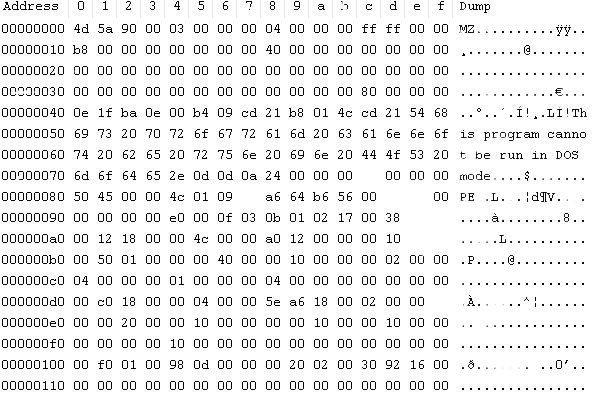
\includegraphics[width=1.0\textwidth]{hex.png}
	\caption{Hexadecimal view of malware}
	\label{hexview}
  %\vspace{-4mm}
\end{figure}

See Fig.~\ref{asmview}. Before getting to the source code, malware binaries must be taken apart. Most of the time, tools like Interactive Disassembler (IDA)~\cite{78}, Radare~\cite{79}, Ghydra~\cite{80}, and others are used. To make a good classifier, we suggest taking hand-crafted features from both the hex view and the assembly view of the executable. This way, we can use the complementary information that these two views provide. More specifically, we chose to limit our proposed method to only common and well-known features~\cite{24}~\cite{77} so that we could see if the system's ability to classify things got better after adding deep features that were found using deep learning models. After that, the malware's hexadecimal source code and assembly language source code are used to show the features that were made by hand.
\color{black}
\begin{figure}[tb]
	\centering
	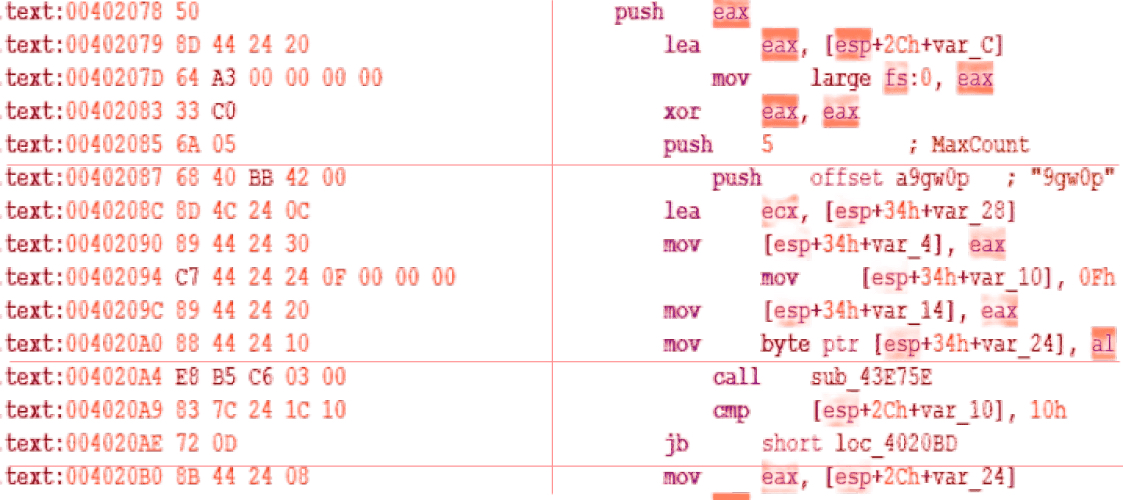
\includegraphics[width=1.0\textwidth]{assembly.png}
	\caption{Assembly view of malware}
	\label{asmview}
  %\vspace{-4mm}
\end{figure}

Grayscale images can be converted from raw malware executable files showing features of malware~\cite{13}~\cite{11}. Grayscale images can capture minor changes without altering global structure of the data and also has lower computational requirements. Nataraj et al.~\cite{11} originally used byte plot visualization as grayscale pictures to classify malware images. \%9,342 pictures of 25 types of malware were included in the sample.  
They retrieved and evaluated GIST characteristics from grayscale images using K-nearest neighbor classification and Euclidean distance as a performance metric. However, their method was computation intensive. Mirza et al.~\cite{15} extracted properties from malicious files to identify malware using decision trees, support vector machines, and boosting methods. Zhang et al.~\cite{16} categorized ransomware using n-grams of operation codes through a static analysis. Makandar and Patrot~\cite{38} used a multi-class SVM to detect malicious input with texture-based feature vectors from malicious images. They used a wavelet transform to reduce the dimension of feature vectors and computational cost. However, traditional machine learning approaches require features that are completely dependent on experts' design. As a result, local features that are significant to malware creation remains unnoticed. 

Researchers working with malware classification problem have used Convolutional Neural Network (CNN) architectures. The main advantage of using CNN on graysacle images is to extract hidden features and also analyze similar behaviour among malwares belonging to the same families. Cui et al.~\cite{17} identified harmful code changes using a basic CNN model and grayscale images. Kalash et al.~\cite{07} identified malicious images by translating malware binaries into images and then fed the images into a CNN. This enhanced malware detection process and the accuracy was 98.52\% and 98.97\%, respectively, for benchmark datasets. Yue's~\cite{18} weighted softmax loss for CNNs classified imbalanced malware images and achieved satisfactory results.  Gilbert et al.~\cite{19} used a  network of three convolutional and one fully connected layers to improve the classification performances significantly. Gilbert's work validated against the MalImg and Microsoft Malware Classification Challenge datasets. Vinayakumar et al.~\cite{22} suggested a CNN-LSTM deep learning network to classify malware families. 

% Tobiyama et al.~\cite{21} suggested Recurrent neural networks (RNNs) to extract activity features of a process and subsequently use a CNN to classify them. 
 

% \textcolor{blue}{MalImg experiments showed 96.3\% accuracy on the mentioned experiment}. \textcolor{blue}{Su et al.~\cite{23} identified one-channel grayscale pictures using a lightweight CNN from two types of executable binaries with a detection accuracy of malware being 94.0\% and goodware being 81.8\%}.

In classifying malware images using Convolutional Neural Network (CNN) Models~\cite{28}, authors used a variety of CNN models to categorize a malware family. Three of the six deep learning models that they employed have previously won the \text{ImageNet Large-Scale Visual Recognition Challenge}. The remaining three models, CNN-SVM, GRU-SVM, and MLP-SVM, augment neural models with SVM. They assesed their approach with MalImg~\cite{10} dataset that comprises with malware images derived from PE malware programs. The collection contains 25 families of malware. The Inception $V3$ model outperforms the M-CNN model proposed by Kalash~\cite{07} , with a test accuracy of 99.24\% vs 98.52\%.

In~\cite{25}, Gibert et al. offer a hybrid method for malware classification in lieu of training gradient boosting trees. The method involved combining deep or hidden and hand-crafted features~\cite{25} to increase the number of features extracted. This model outperforms every deep learning and feature based approaches in the literature when evaluated using the dataset obtained from Microsoft Big Data Innovation Gathering Challenge (2015), denoted as Microsoft Big. \color{blue} However, multi-modal systems like HYDRA prove to be very resource-intensive and prone to Concept Drift. Since malwares can constantly be replicated through obfuscation, variety of features used here can become obsolete.   
\color{blue} \par In MalFCS \cite{27}, malwares are visualized as entropy graphs based on structural entropy. No further decomposition or decryption of malware files are done. CNN is used for detection of patterns similar to malware families in the entropy graphs. The mentioned model achieved an accuracy of 99.7\% and 100\% on MalImg and Microsoft dataset respectively. But the lake of transformation knowledge of images from binaries sometimes may vary for generating malware and can differ the accuracy from the original one.
\par
\textcolor{blue}{Deep CNN architecture was employed in Deep Transfer Learning for malware image classification in the DTMIC~\cite{34}. Following the feature extraction from the convolutional layers, features are single-vectorized and fed into a fully connected dense layer. Then, a regularization technique known as Early Stopping monitors the validation loss to minimize the overfitting problem. DTMIC outperformed the existing approaches and was resistant to compressed and encrypted malware. It obtained test accuracy of 98.92\% for MalImg dataset and 93.19\% for Microsoft dataset}. 
\par
 \textcolor{blue}{ In \cite{39}, visual recurrences among the malwares belonging to the same family has been exploited for malware detection. Here, for increasing sample sizes and to deal with imbalanced dataset, image augmentation has been used. For in depth feature extraction of the images, convolutional and maxpooling layer of VGG16 network is utilized. The output from VGG16 network is then passed to a BiLSTM network for extracting latent structural features of the images. BiLSTM processes the derived features from VGG16 sequentially which is crucial for extracting patterns from images. The two mentioned models are stacked and the final classification result is obtained by passing the output of ensembled model into a dense layer.  When tested against MalImg and Big2015 dataset, accuraccies of 99.56\% and 98.56\% respectively were obtained. However, their image augmentation techniques that involve shifting, flipping and rotating the images may remove bytes, leading to obscuring more features that could have been detected.}
 %\begin{figure}[ht]
	%\centering
	%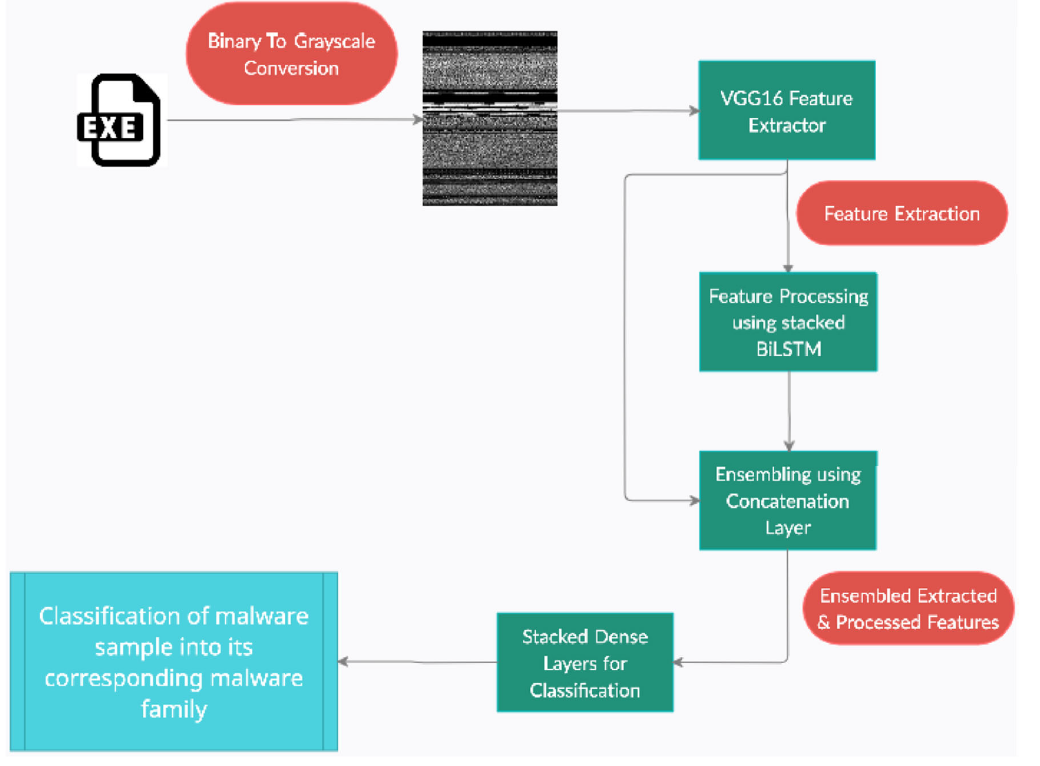
\includegraphics[width=0.5\textwidth]{Conrec.png}
	%\caption{ConRec}
	%\label{conrec}
  %\vspace{-4mm}
%\end{figure}
\par
 \textcolor{blue}
A new deep-learning framework based on hybrid model has been adapted in \cite{40}. For tackling adversarial attacks, the feature vector of 4096 dimensions is prepared using two pre-trained networks, ResNet50 and AlexNet. Next, using softmax layer the final classification has been done. Feature extraction process involves transfer learning in this work. Tested against MalImg and Microsoft Big 2015 dataset, the mentioned framework has an accuracy of 97.78\% and 94.88\%
respectively. However, no approach for resolving data imbalance has been adopted in this paper.  
%\begin{figure}[ht]
	%\centering
	%\includegraphics[width=0.5\textwidth]{deepLearningFramework.png}
	%\caption{Deep Learning Framework}
	%\label{newDeepLearningFramework}
  %\vspace{-4mm}
%\end{figure}

\color{black}
\par
The approaches explained above sometimes tweaks the dataset, which can cause removal of concealed features.
A lot of information hidden in the malware may get ignored in this way. Our work surpasses this challenge uniquely by using spatial information from an image to find patterns hidden in deep  
learning models for malware classification.  \color{blue}Besides, the image augmentation process described in our approach has least data loss.  
\color{black}
\section{Proposed Approach}
\label{approach}

By effectively finding malware families, our model can detect subtle modifications. Also it can extracts deep features by incorporating local properties utilizing a simple, but effective method. At first, the bytes are represented as three channels grayscale images. Secondly, if required, the images are adapted to an appropriate augmentation. Then, to extract deep characteristics from raw pixel data, a spatial convolutional neural network is implemented followed by the implementation of a classical CNN architecture. The whole architecture is then used to automatically train the classifier. Finally, a dense layer with sufficient regularization is provided to complete the connectivity for categorizing malware families. In Fig.~\ref{fig_ourProposedSystem_1},We demonstrate our proposed classification approach.

\begin{figure}[tb]
	\centering
	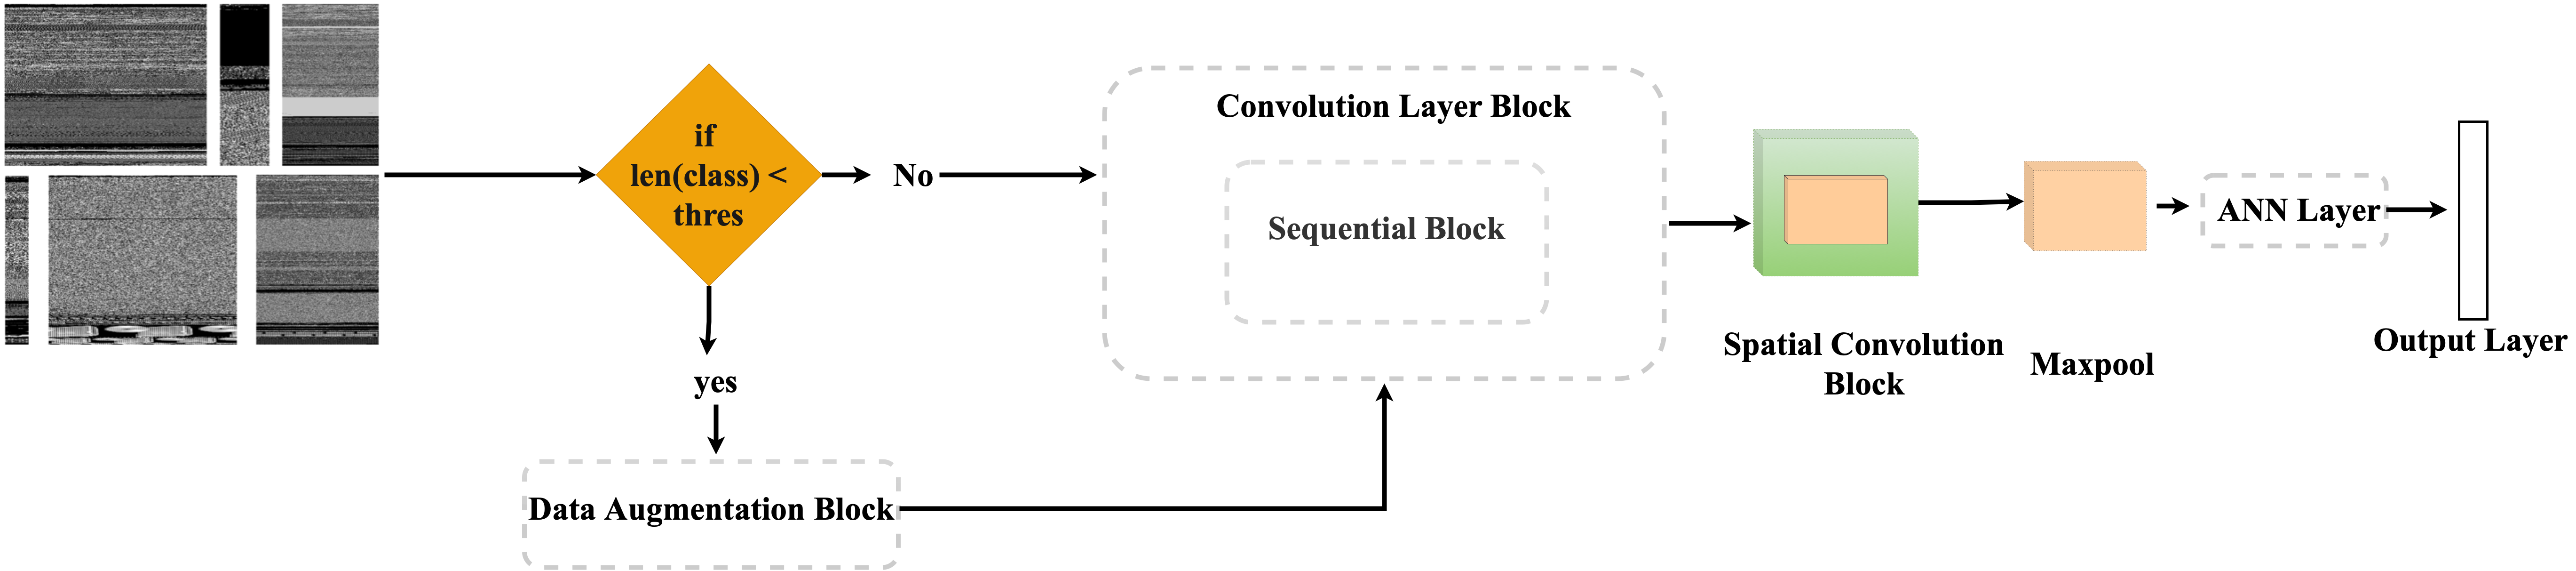
\includegraphics[width=1.0\textwidth]{Full-flow-2.png}
	\caption{Our Proposed System}
	\label{fig_ourProposedSystem_1}
  %\vspace{-4mm}
\end{figure}

\subsection{Image Generation from Portable-Executable file}
While dealing with malware, only reading the sequence of binary for malware data is not worthy to find out the criteria of  attack. The binary sequence converted to an image is better suited for CNN-based architecture. In the process of image construction, at first, malware executable binary (PE) file is segmented as a sequence of bytes. Each byte represents a decimal number (range $0$ to $255$). The numbers constitute a decimal vector representation, that is converted into a malware image sample afterwards. For each row of the image binary, we construct a set of vectors that forms a $2-D$ matrix. The matrix is then converted into three channel ((R)ed, (G)reen, and (B)lue) image. We applied the following widely accepted technique for changing RGB ((R)ed, (G)reen, and (B)lue) images to grayscale ones is: $\displaystyle    g_i = 0.299 \times r_i + 0.587 \times g_i + 0.114 \times b_i$

Fig.~\ref{imagegeneration} depicts the process of image representation. Note that, each grayscale malware image width is $256$ pixel, but the height is variable depending on size of each malware.
\begin{figure}[tb]
	\centering
	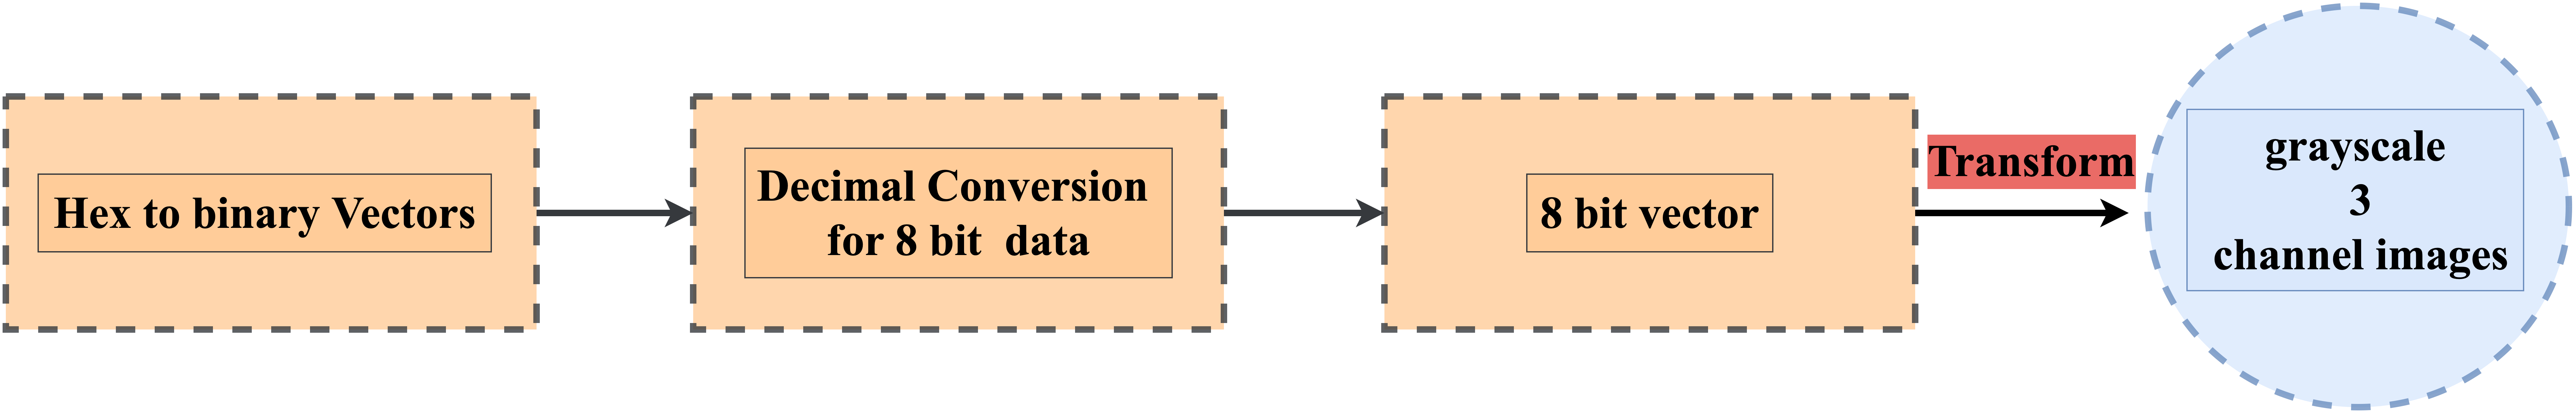
\includegraphics[width=1.0\textwidth]{image transform.png}
	\caption{Malware Image generation from PE file}
	\label{imagegeneration}
  %\vspace{-4mm}
\end{figure}

\par
So as shown in Fig.~\ref{grayscale}, Some malware images represented below as a gray scale.The ability to distinguish between the various parts of a binary is the key advantage of viewing a malicious binaries as an image.

\begin{figure}[h]
  \centering
 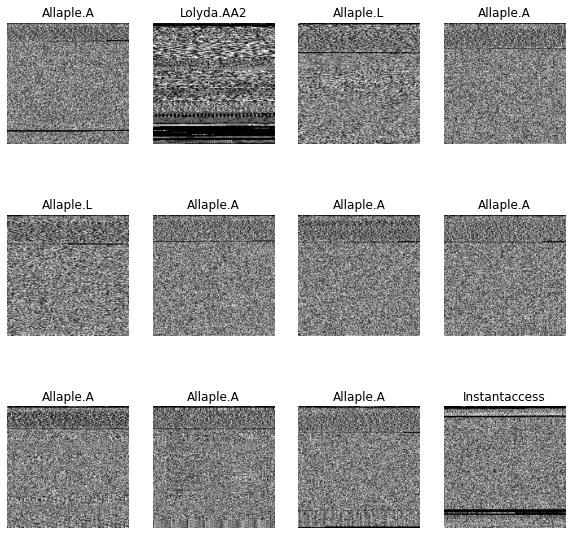
\includegraphics[width=1.0\textwidth]{grayscale.png}
  \caption{ Gray scale images of malicious binaries}
  \label{grayscale}
\end{figure}

\subsection{Image Augmentation}
\label{augmentation}
Once the malware files are converted in to images, we checked for the imbalance trend of the dataset. Since, imbalanced datasets can cause over-fitting or under-fitting in classification, we utilized image augmentation to deal with this problem. Existing augmentation techniques, such as (a) flipping, (b) rotating, and (c) shifting may alter the data by removing or changing some patterns and order of the bytes. Therefore, we adopted a strategy for image augmentation (as shown in Fig.~\ref{dataaug}) using a Generative Adversarial Network (GAN) that can produce pseudo images for less sample classes in the dataset to balance the distribution of classes.

In the cycleGAN (Fig.~\ref{dataaug}), new images are generated utilizing two discrete, unpaired images. The cycleGAN technique eradicates disproportional hallucinations of image features and prevents unnecessary data loss through cycle consistency. Note that data loss is measured through a detrimental metric, named L2-loss, to our image generation procedure.

\color{blue}
The optimal convolutional dimension which is used in discriminator and generator block are actually found by experiment. In our optimal hyper parameter for discriminator is : $64$, $128$, $256$, $512$ and for generator is : $64$, $128$, $256$. 
\color{black}


\begin{figure}[tb]
	\centering
	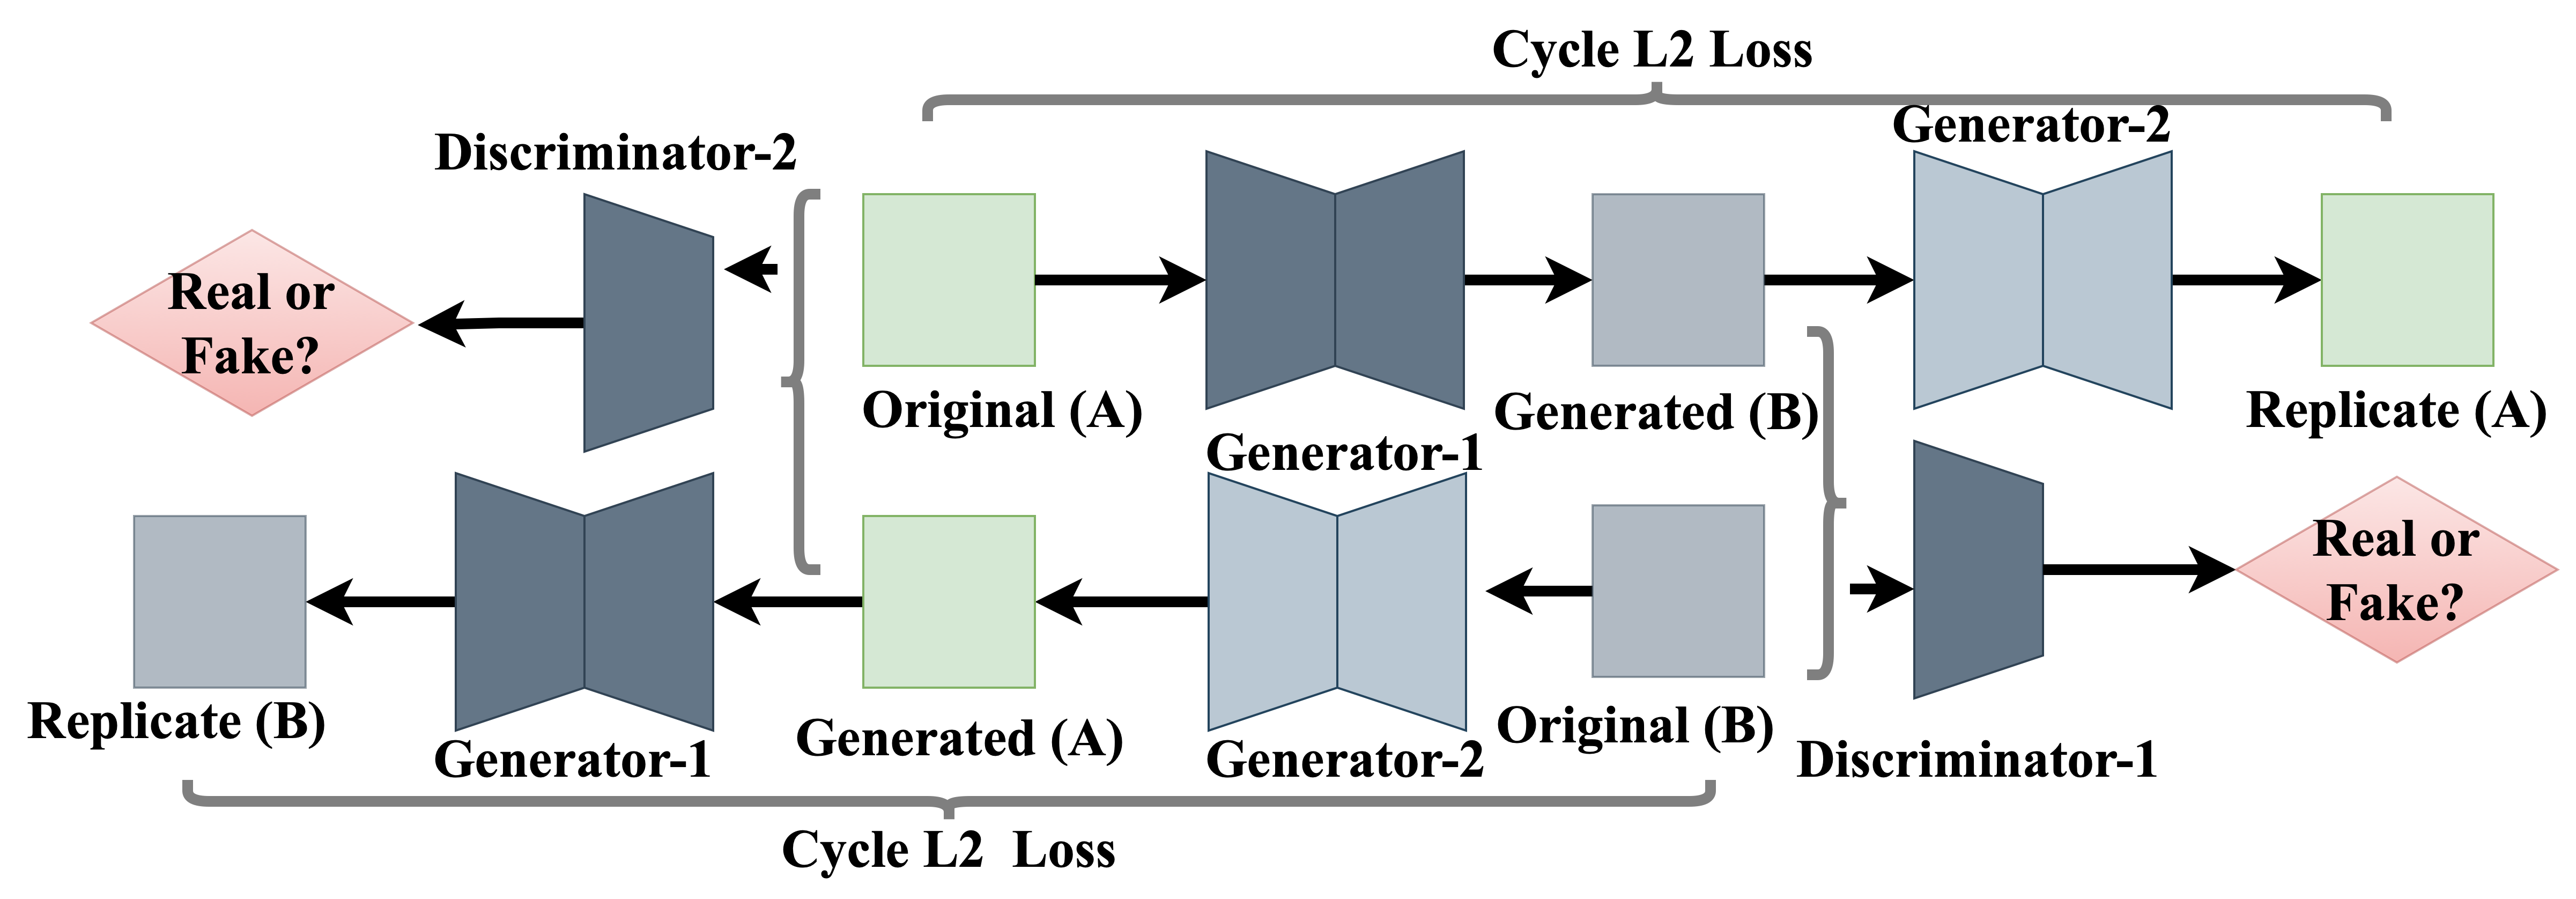
\includegraphics[width=1.0\textwidth]{data-aug.png}
	\caption{Image Augmentation with cycleGAN}
	\label{dataaug}
  %\vspace{-4mm}
\end{figure}

\subsection{Classical Convolutional Neural Network Block}
Our Classical Convolutional Neural Block is very simple and lightweight for extracting important features from malware images. It consists of $2$ convolutional layers and $2$ maxpool layers. Convolution layer is important for extracting features and maxpool layer is responsible for transforming high-dimensional features into low-dimension features by reducing the number of pixels utilizing max values of the matrices obtained from convolutional layer. Before feeding into the convolutional layer, the augmented images should be resized and re-scaled to reduce the number of parameters in training. Fig.~\ref{ClassicalCNN} displays the classical CNN Block in our system with appropriate shape.

\begin{figure}[ht]
	\centering
	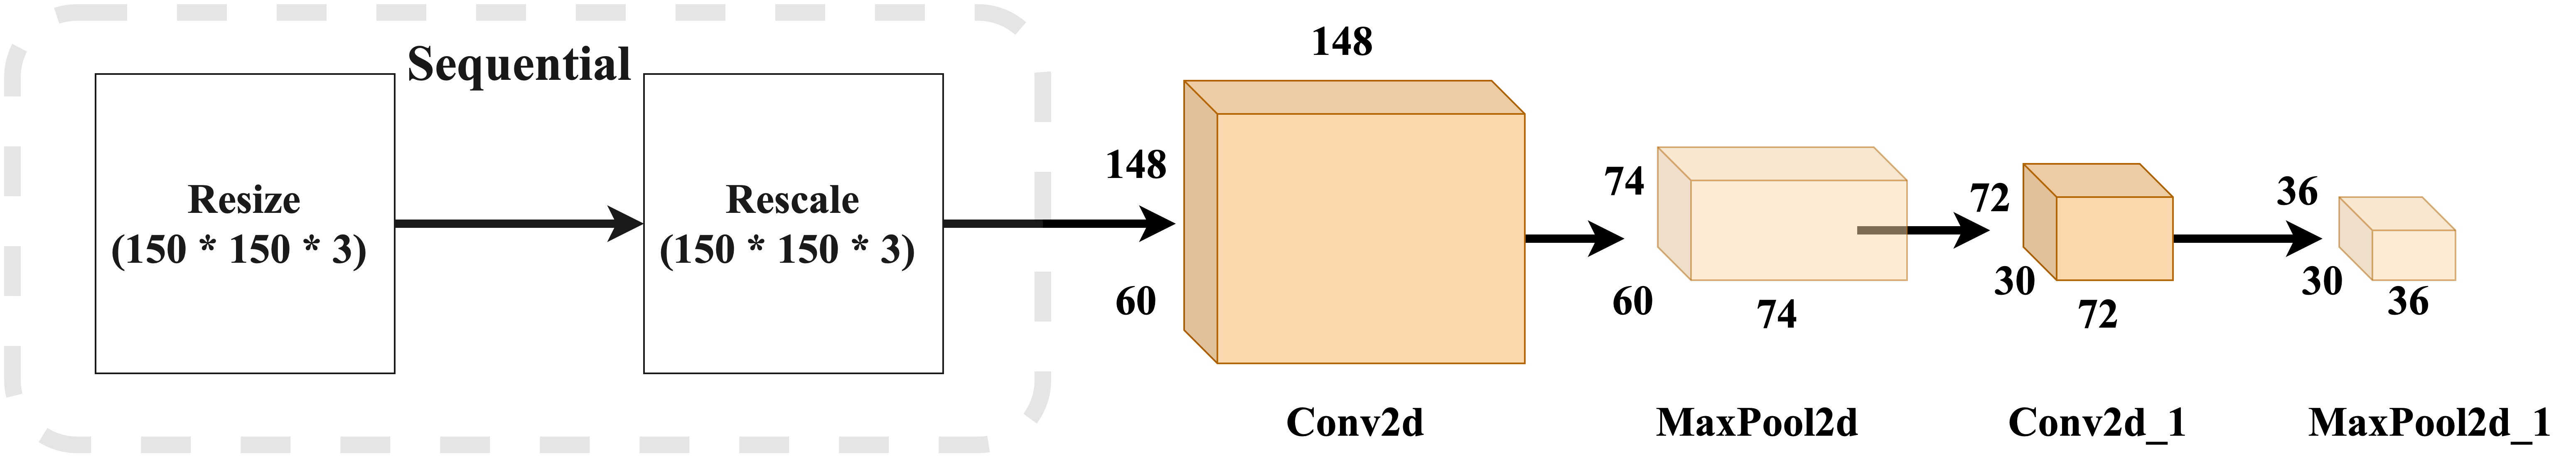
\includegraphics[width=1\textwidth]{sequential.png}
	\caption{Classical CNN Block}
	\label{ClassicalCNN}
	% \vspace{-4mm}
\end{figure}

\color{blue}
In Fig.~\ref{ClassicalCNNlayer} depicts the layer visualization for Fig.~\ref{ClassicalCNN}. The specified layer is performs well for our proposed system which can be found by trial and error technique.

\begin{figure}[ht]
	\centering
	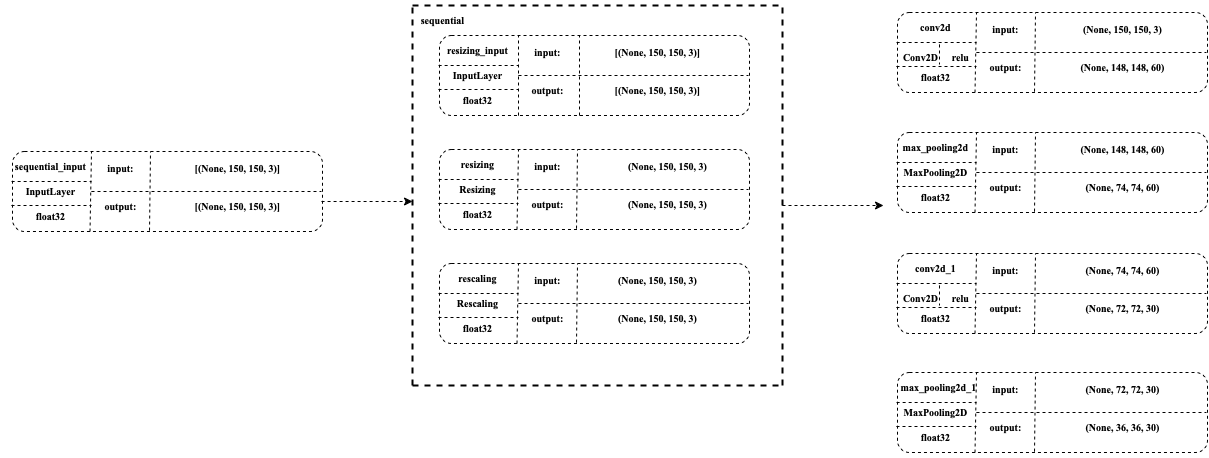
\includegraphics[width=1\textwidth]{CNN.drawio-2.png}
	\caption{Classical CNN Block}
	\label{ClassicalCNNlayer}
	% \vspace{-4mm}
\end{figure}

\color{black}
\subsection{Proposed Spatial Convolutional Network (Sp-CNN)}
Our goal is to develop a CNN that understands the context of images in terms of their spatial connection to one another. Different types of malware use distinctive patterns of pixels in their binary representations. In order to categorize malware families, deep learning must be used to extract the deep information, i.e., features, associated with pixel layouts. Our proposed SCN is used to extract such features. The term ``spatial'' used in  ``Spatial attention channel'' should not be confused with the term ``spatial '' in the proposed SCN. Since, in SCN, spatial information is propagated via a specifically built CNN. 

Fig.~\ref{SpCNN} shows the proposed Spatial Convolutional Neural Network (Sp-CNN) module. It is applied on a three  dimensional tensor of size \({Channel}\times{Height}\times{Width}\), where $Channel$, $Height$, and $Width$ denote the number of depths, rows, and columns of a tensor obtained from previous MaxPool layer, respectively. The tensor must be divided into $n$ slices where each slice goes through a spatial convolutional layer with $p$ kernels of shape ${p} \times {w}$, where $n$ and $p$, respectively, are equal to the height and number of channel of the previous classical CNN layer, and kernel width is represented as $w$ ($w \in Width$). Note that the slices are performed to extract features from different data segment of a malware binary in order to more effectively capture the information of the family of malware. In particular, a symmetric kernel is passed to the next layer in a classical CNN as an outcome of some operations in the current layer. On the other hand, in our approach, we update each of our slices using an asymmetric kernel. While passing each of the slices through a spatial CNN, an modified slice is obtained through the summation of kernel operation. The process of altering the slices through every layer repeated until the final slice is updated. All modified slices are then passed to the next Sp-CNN layer.

We obtained empirically that applying ``Sp-CNN'' on the top of hidden convolutional layer provides the best outcome because the top most layer contains more reliable information. It is also a better starting point to pull out spatial relationships due to the amount and reliability of information.

\subsection{Feed Forward ANN}

We have used five fully connected components at the end of our spatial network (as shown in Fig.~\ref{ANN}) for multi-class categorization. After applying our spatial network to the  top of our convolutional network, we use a maxpool $(2,2)$ to reduce the dimension of the feature maps. The dimension reduction of the features, performed before applying any dense layer followed by hidden layers, is preferable and performed to prevent the over-fitting. Three hidden layers which have $256$, $128$, and $50$ neurons, respectively, and an output layer is implemented in our classifier block (see Fig.~\ref{ANN}). The size of output layer varies depending on the total number of classes used in our dataset. 

We have utilized ``RELU'' as an activation function and also a ``dropout'' is used as a regularization method with $0.2$ as input parameter in each dense and hidden layer for predicting malware families. In order to avoid overfitting, the dropout layer periodically resets input units to $0$ during the training. All inputs are multiplied by $\frac{1}{1 - 0.2}$ to keep the sum over all inputs unchanged. At the very last layer, the ``softmax'' activation function is used to select the class with the largest probability.
\color{blue}
All the hidden layer block size can be found by trial and error mechanism which can produce optimal result for our all dataset when evaluated.
\color{black}

\begin{figure}[ht]
\centering

        \centering		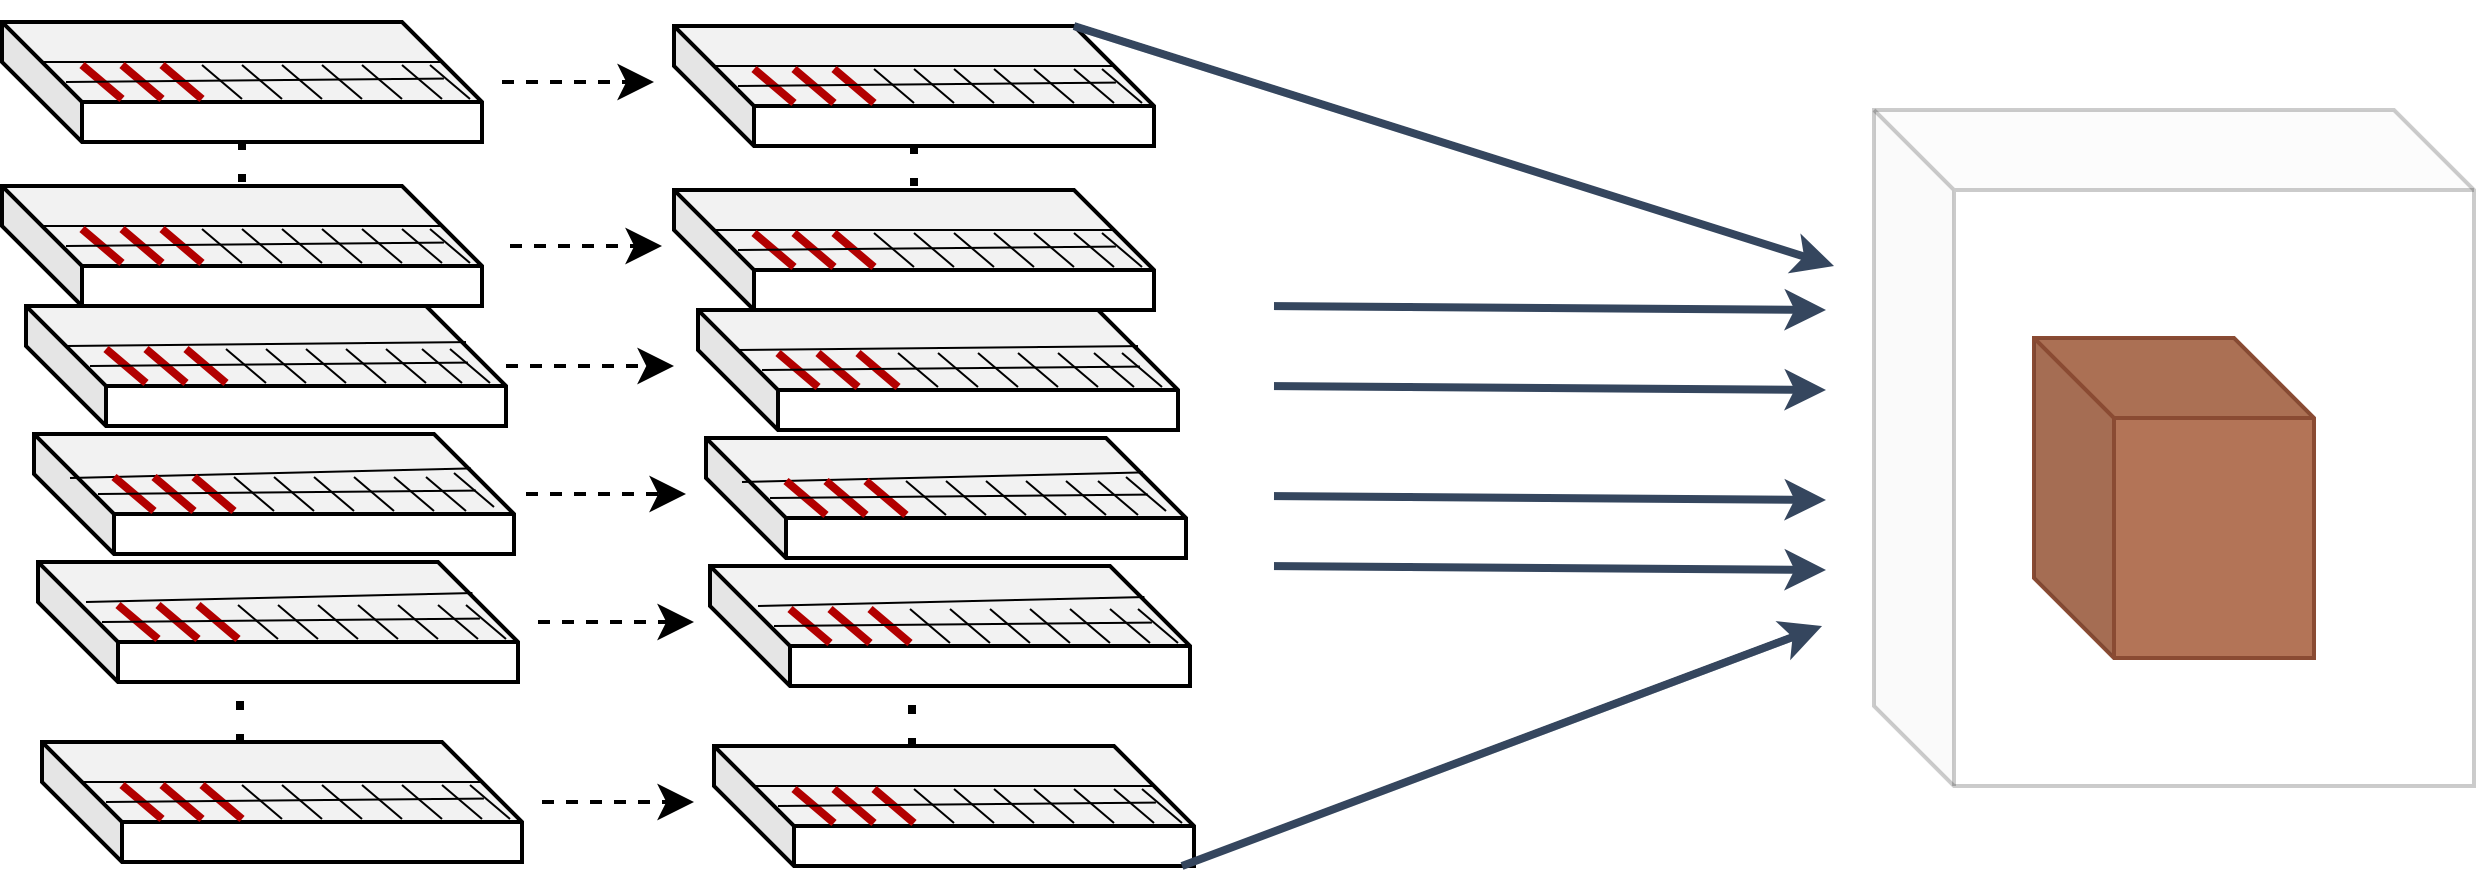
\includegraphics[width=1.0\textwidth]{Spatial-2.png}
	    \caption{Spatial Relationship Extractor (Sp-CNN)}
	    \label{SpCNN}
		\end{figure}
  
\begin{figure}[ht]
        \centering
		\hspace*{0.1in}
		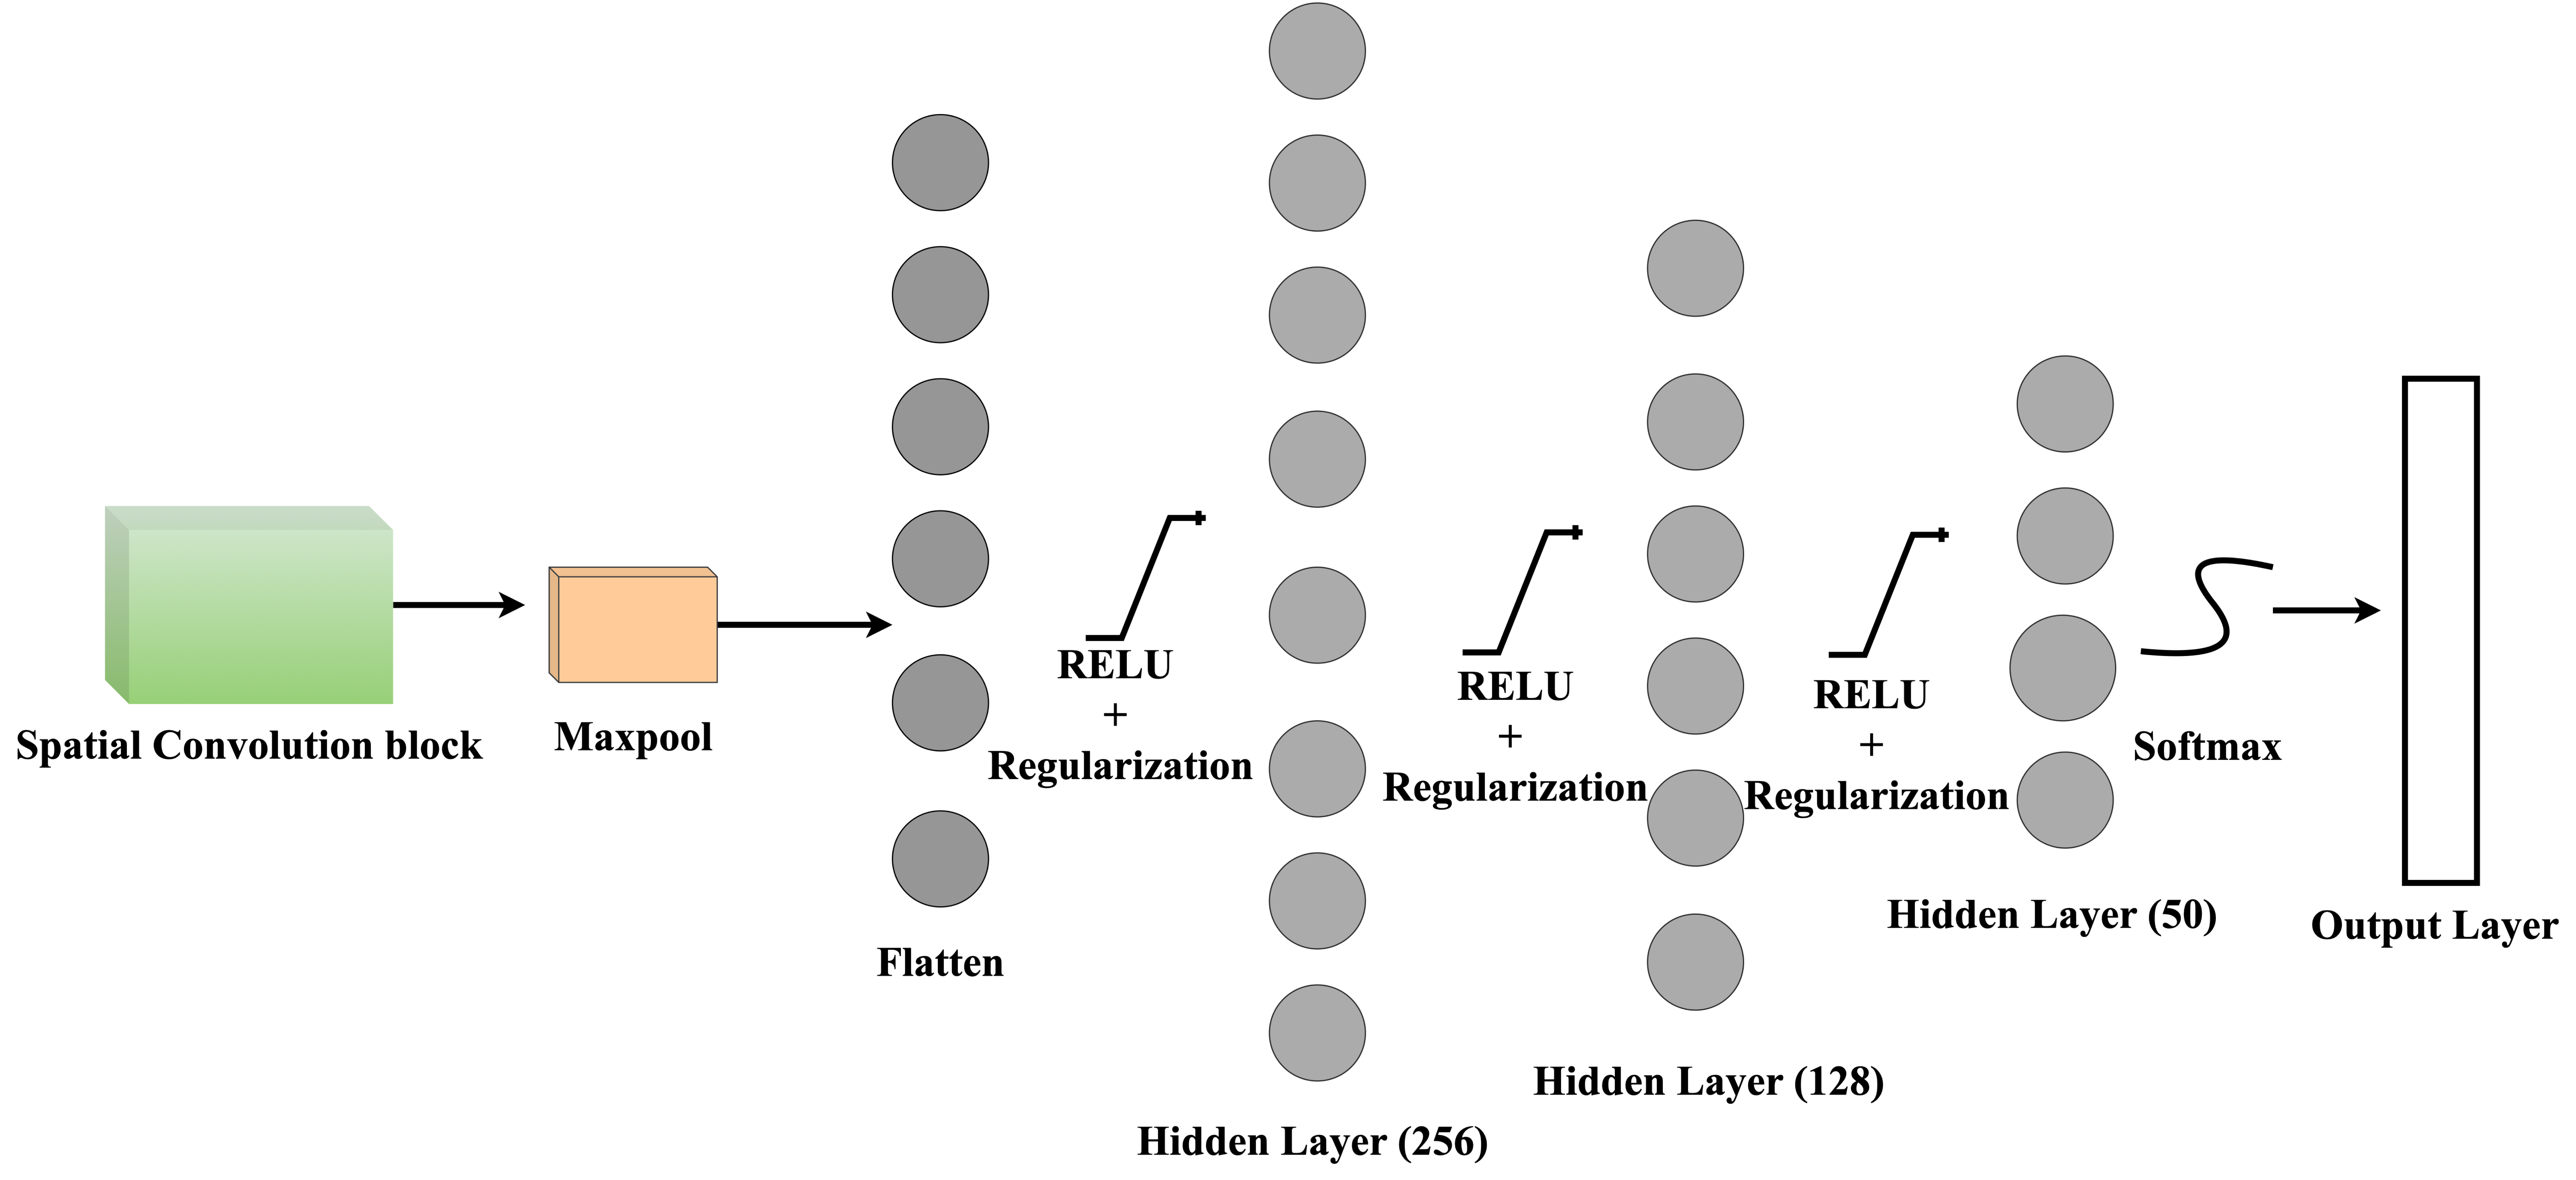
\includegraphics[width=1.0\linewidth]{ANN.png}
	    \caption{Feed Forwarded Network}
	    \label{ANN}
		
   \vspace{-4mm}
	\end{figure} 

\section{Empirical Evaluation}
\label{Analysis}
Our system is run on a server with a 32GB RAM, a CPU from Intel's 8th generation Core family, a GPU from Nvidia's RTX2080 Ti Max Q Design, and 16 GB of video memory. We have used Tensorflow-keras as backend to construct our model.

We adopted $k$-fold cross validation, where $k = 10$, to evaluate the performance of our model. Every dataset used in $k$-fold validation is split into $k$ equal samples. Then, each of the $k$ samples is further splitted into $k$ sub-samples to use $k-1$ sub-samples for training and the remaining one sub-sample for validation. We calculate the mean of the accuracies obtained from all the folds and assess the model using the test set.

% \subsection{Dataset}
% \label{dataset}
\subsection{Dataset}
\label{dataset}
We have used some well-known datasets used for malware classification, such as, MalImg~\cite{11}, \text{Microsoft Malware data}~\cite{10} and Malevis~\cite{39}. The MalImg dataset consists of different malware images that were converted from malware binaries a.k.a PE. In this public dataset, there are 9,339 samples belonging to 25 families. In the \text{Microsoft Malware data}~\cite{10}, is the most used benchmark dataset for classifying malwares. It includes half terabytes of data consisting of 10,868 samples. \textcolor{blue}{Another dataset, namely Malevis~\cite{39}, provided by Hacettepe University, containing 14,226 samples divided into 26 (25+1) classes. Here, only one category reflects ``legitimate'' samples, whereas the other 25 categories describe different types of malware.}
Class imbalance is present in the benchmark datasets except Malevis that we have used for evaluating our model. Fig.~\ref{fig:def1} and Fig.~\ref{fig:def2} show the imbalance distribution for MalImg and Microsoft samples, respectively. 
While the existence of imbalanced classes in the datasets are a drawback, they are nevertheless useful for evaluating the efficacy of various machine learning strategies applied to malware classification. We resolved the data imbalance problem through the data augmentation approach as discussed in the Section~\ref{augmentation} that balances the number of training samples for each category.

\begin{figure}[h]
\centering
        \centering
		
		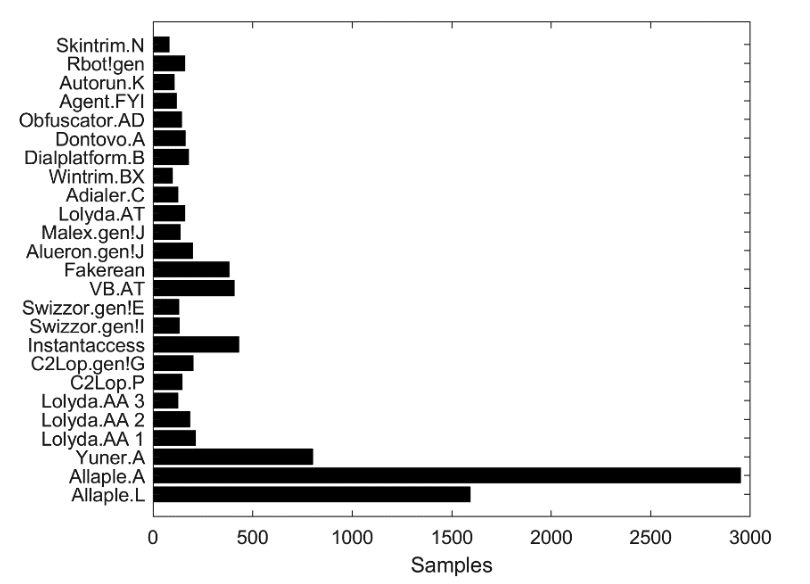
\includegraphics[width=1\linewidth]{malimg-2.png}
		\caption{ Distribution of MalImg Samples}
		\label{fig:def1}
	   \end{figure}
		\begin{figure}[h]
        \centering
		
		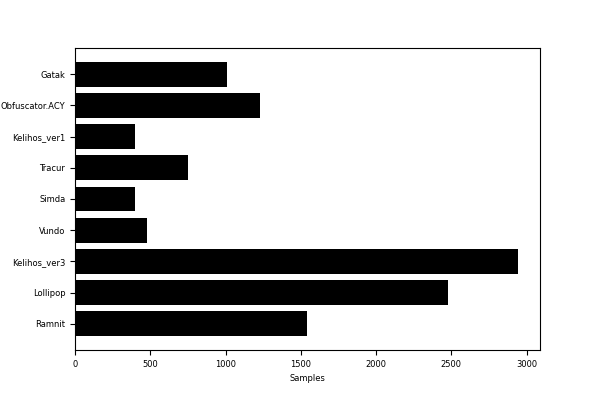
\includegraphics[width=1\linewidth]{microsoft-distrib.png}
		\caption{ Distribution of Microsoft Samples}
		\label{fig:def2}
   \vspace{-4mm}
	\end{figure}

 \textcolor{blue}{Another collection of images synthesized by APKs is used for our experiment. After that, images are assigned a label denoting whether they are benign or malware for binary classification purposes. Thirteen thousand malicious applications and five thousand benign applications were used for feeding our model. On those  thirteen thousand malicious programs, 5,000 of which are from the old DREBIN\cite{45} dataset and the remainder from ANDROZOO's \cite{44} website including benign values. As we are collecting images from different sources, we can give a name for this dataset as ``Android Malware Dataset''. In Table~\ref{dataset}, An overview of all dataset which is evaluated in our proposed method is given.}
 	\begin{table}[tb]
         \centering
		 \caption{All Dataset Overview in our Proposed System}
		 \begin{tabular}{|p{2.5cm}||p{0.9cm}||p{1cm}||p{1.2cm}||p{1cm}||p{1.2cm}|}
			\midrule
			\textbf{Dataset Name} & \textbf{Source} & \textbf{URL} & \textbf{Notation} & \textbf{Number of Classes} & \textbf{Number of \text{Samples}}\\\\
			  \midrule
			malimg\_dataset9010  &  \cite{11} & \cite{81}  & MalImg & 9,339 & 25 \\\\
		
			BIG 2015 & \cite{10} & \cite{82} & Microsoft Big & 10,868 & 9 \\\\
			
			MaleVis Dataset & \cite{39} & \cite{83} & MaleVis & 14,226 & 26 \\\\
	
			DREBIN \& ANDROZOO &  \cite{44} \cite{45}  & \cite{84} \cite{85} & Android Malware Dataset & 14,226 & 2 \\\\
			\hline
		\end{tabular}
	
		\label{dataset}
  \vspace{-4mm}
	\end{table}

\subsection{Performance Metrics}
We have used two performance metrics to assess our proposed  approach, namely accuracy and macro $f1$. The percentage of successful predictions is simply known as accuracy. 
% The formula for accuracy can be defined as :\\$\displaystyle
%          Acc  = \frac{\#\;Correct\;Pred}
%          {Total}
% $
A multi-class logarithmic loss ($logloss$) is used while evaluating the performance using the metrics. We used the cross entropy between the ``true" label and the anticipated probability as the logarithmic loss, denoted as: $\displaystyle
logloss = -\frac{1}{N}\displaystyle\sum_{i=1} ^{N}\displaystyle\sum_{j=1} ^{M}Y_i,_jLOG(P_i,_j)
$
However, measurement of accuracy is not always a good criterion for evaluating the resilience of ML models in datasets with a higher degree of imbalance. Hence, we have also considered the $f1$ score of each class. In order to determine an overall $f1$ score for a dataset containing more than one class, we need to aggregate all the calculate $f1$ scores in some way. Macro-$f1$ score is the unweighted mean of the $f1$ score calculated per class and  the simplest aggregation for $f1$ score. Formal representation for Macro-$f1$ used in our evaluation is defined as: $\displaystyle
\text{Macro-$f1$}  =  \frac{1}{N} \sum_{i=0}^{N} {\text{f1}_i}$,
where
$\displaystyle
\text{${f1}_i$}  =  2 \cdot \frac{\text{Precision} \cdot \text{Recall}}{\text{Precision} + \text{Recall}}$, for $i$ being the class which is being evaluated and $N$ being the total number of classes.

\subsection{Hyperparameter}
% \label{parameter}
%{\bf Hyperparameter:}
The model is trained over a period of about 30 epochs. For all the datasets, we have used similar hyperparameter values as that of our training samples for the sake of consistency of our model. Adam optimizer with a learning rate of $1.6\mathrm{e}-4$ and sparse categorical cross entropy loss function have been used to configure our model. The size of input images after augmentation and before feeding into the network is ${150} \times {150}$, while the batch size is $32$. 
Table~\ref{hyperpara} shows all the hyperparameter values that are used for training our network for all datasets. We have determined precise values for these hyperparameters on trial-and-error basis because optimization approaches and procedures require additional computational expenses. Moreover, this strategy is rigorous and has been widely employed in a range of recent research delivering ML and DL-based solutions.
%\vspace{-3mm}
	\begin{table}[tb]
         \centering
		 \caption{Optimized Hyperparameter for our proposed method}
		 \begin{tabular}{|p{2.6cm}||p{1.5cm}||p{4cm}|}
			\midrule
			\textbf{Training-hyperparameter} & \textbf{Values} & \textbf{Description} \\\\
			  \midrule
			Batch size  &  32 & iterative training examples per epoches.  \\\\
		
			Cross validation & 10 & Statistical method for comparing learning algorithms by separating data into training and validation segments. \\\\
			
			Epoches &  30 & One cycle of neural network training. \\\\
	
			Image resize &  \({150} \times {150}\) & critical pre-processing step in computer vision \\\\

            Learning rate  & 1.6e-4 & A tuning parameter in an optimization method that determines step size during iterations while moving toward a minimum of a loss function. \\\\

            Optimizer & Adam & A function or method that adjusts neural network weights and learning rate. \\\\

            Loss function  & Sparse Categorical Cross Entropy & A way to measure how effectively your algorithm models your data. \\\\

            Monitor & Validation accuracy & monitoring and evaluating production model performance to verify use case quality. \\\\
			\hline
		\end{tabular}
	
		\label{hyperpara}
  \vspace{-4mm}
	\end{table}
\subsection{Experimental Results}
\label{result}
The fundamental objective of our proposed method is to accurately identify and classify malware families. While training, a $10$-fold cross-validation is utilized to improve model performance.


\begin{table}[tb]
     \centering
	\caption{train and cross validation accuracy}
	\begin{tabular}{|p{2cm}||p{1.5cm}||p{1.2cm}||p{2cm}||p{1.5cm}||p{1.2cm}|}
		\midrule
		\multicolumn{3}{c}{\textbf{MalImg}} & \multicolumn{3}{c}{\textbf{Microsoft Big}}\\
          \midrule
		\textbf{} & \textbf{Train(\%)} & \textbf{Val(\%)} & 
  \textbf{} & \textbf{Train(\%)} & \textbf{Val(\%)}\\\\
		\midrule
		\textbf{iteration 1}  &  77.75 & 95.81 & \textbf{iteration 1}  &  71.80 & 91.91\\\\ 
	
		\textbf{iteration 2} & 94.78 & 97.15 & \textbf{iteration 2} & 89.74 & 93.47\\\\
	
		\textbf{iteration 11} &  98.93 & 97.67 & \textbf{iteration 11} &  98.86 & 99.54 \\\\
		
	\textbf{iteration 16} &  99.88 & 99.83 & \textbf{iteration 16} &  99.70 & 99.63  \\\\
		
		\textbf{iteration 18}  & 99.89 & 99.88 & \textbf{iteration 28}  & 99.89 & 99.63 \\\\
		
		\textbf{Final} & 99.95 & 99.93 & \textbf{Final} & 99.92 & 99.72\\\\
  	\hline
	\end{tabular}
	\label{iteration}
\vspace{-2mm}
\end{table}

Table~\ref{iteration} demonstrates the accuracy attained while training our model using the benchmark datasets adopting a $10$-fold cross-validation technique. In Table~\ref{metric}, all the metric values that are necessary for the assessment of our model utilizing MalIMG and Microsoft test-sets of data are presented.

\begin{table}[tb]
    \centering
	\caption{Performance Result for our Proposed Method}
	
	\begin{tabular}{|p{2cm}||p{1.5cm}||p{1.5cm}||p{2cm}||p{1.5cm}||p{1.5cm}|}
		\cmidrule{1-6}
		\textbf{Metric} & \textbf{MalImg} & \textbf{Microsoft BIG} & \textbf{Metric} & \textbf{MalImg} & \textbf{Microsoft BIG}\\
        \cmidrule{1-6}
		Precision(\%)  &  99.92 & 99.93 & F1(weighted) &  99.96 & 99.92 \\\\
		Recall(\%) & 99.84 & 99.71 & Test-Acc(\%)  & 99.87 & 99.81\\\\
		F1(macro) &  99.94 & 99.88 & Loss & 0.006 & 0.009\\
		\hline
	\end{tabular}
	\label{metric}
%\vspace{-4mm}
\end{table}

By examining Table~\ref{metric}, we can conclude that our model has achieved 99.87\% test accuracy in MalImg Dataset and 99.81\% in Microsoft Big Dataset. Fig.~\ref{fig:def4} and Fig.~\ref{fig:def5} depict a subset of randomly chosen images, nine for each, for both the test-sets that are classified correctly by our model. Note, the prediction and the confidence values for corresponding images are also shown. 

\begin{figure}[tb]
\centering
    \captionsetup{justification=centering}
    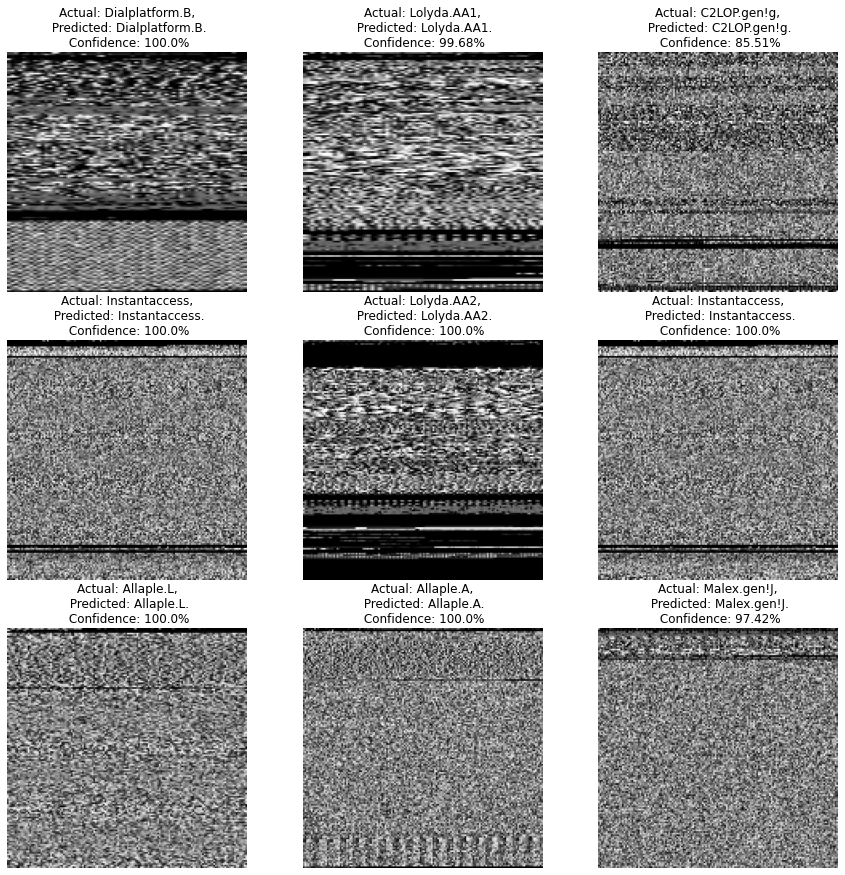
\includegraphics[width=1\textwidth]{malIMG.png}
	\caption{ Random Image's  Confidence score in MalImg Test-set}
	\label{fig:def4}
\end{figure}
 
\begin{figure}[tb]
    \centering
    \captionsetup{justification=centering}
    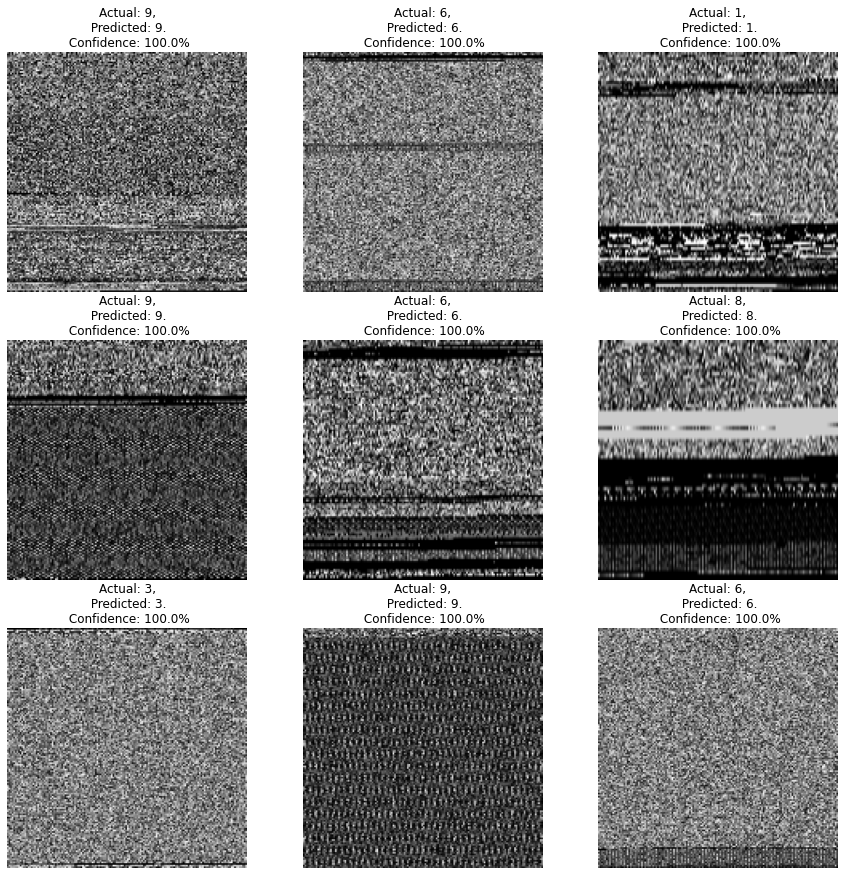
\includegraphics[width=1\textwidth]{big.png}
	\caption{ Random Image's Confidence score in Microsoft BIG Test-set}
	\label{fig:def5}
\end{figure}
	
For clarity, in Fig.~\ref{fig:def5}, Class:9 represents $\xrightarrow{}$ ``Gatak''; Class:6 represents $\xrightarrow{}$ ``Tracur''; Class:1 represents $\xrightarrow{}$ ``Ramnit''; Class:8 represents $\xrightarrow{}$ ``Obfuscator.ACY''; Class:3 represents $\xrightarrow{}$ ``Kelihos\_ver3''.
\par
\textcolor{blue}{In Android Malware dataset, The Dataset contains only benign and malware category. Despite this binary classification, we didn't change our hyper-parameter. In Table~\ref{student-malware} demonstrate the performance of this dataset in our proposed method.}

	\begin{table}[tb]
         \centering
		\caption{Experimental Result in Android Malware Dataset}
		\begin{tabular}{|p{2.6cm}||p{1.5cm}||p{2.6cm}||p{3.8cm}|}
			\midrule
			\textbf{Metric} & \textbf{Values} & \textbf{Metric} & \textbf{Values}\\\\
			  \midrule
			Precision(\%)   &  99.82 & F1(weighted)  & 99.85  \\\\
		
			Recall(\%) & 99.63 & Test-Acc(\%) & 99.72 \\\\
			
			F1(macro)  &  99.86 & Loss  & 0.0076 \\\\
			\hline
		\end{tabular}
	
		\label{student-malware}
  \vspace{-4mm}
	\end{table}

The performance outcome proves that our model is worthy for the most widely acceptable open-source benchmark datasets.


\subsection{Comparative result analysis}
\label{SOTA}
%\noindent
%{\bf Comparative result analysis:}
Here, our technique is compared to the state-of-the-art (SOTA) approaches which comprises feature engineering and Deep Learning (DL). Only the techniques that evaluated their methodology using the Microsoft big \& MalImg datasets were selected to ensure fair comparison.
Besides, in the majority of situations, the existing models and their implementations are not available online or do not function properly, e.g., the parameters must be tuned for the dataset and missing libraries may need to be located. As a consequence, the performance of SOTA approaches are taken from the corresponding original publications for the sake of comparison against our model and shown in 
Table~\ref{comparsion}. 
\begin{table}[ht]
   \centering
	\caption{Comparison with the SOTA Methods for Microsoft Big \& MalImg Dataset. ``-"" represents the corresponding resercher do not mention explicitly about the particular entry of this metrics}
	%{width=0.7\textwidth}
	\begin{tabular}{|p{1cm}|p{0.88cm}|p{0.88cm}|p{0.88cm}|p{0.88cm}|p{1cm}|p{0.88cm}|p{0.88cm}|p{0.88cm}|p{0.88cm}|}
		\midrule
		 \multicolumn{5}{c}{Microsoft Big} & \multicolumn{5}{c}{MalImg} \\
   \cmidrule{1-10}
		\textbf{} & \multicolumn{2}{c}{\textbf{10-fold}} & \textbf{F1-Score} & \textbf{Test} &
  \textbf{} & 
\multicolumn{2}{c}{\textbf{10-fold}} & \textbf{F1-Score} & \textbf{Test}\\
 \cmidrule{1-10}
		\textbf{Method} & \textbf{Acc} & \textbf{LLoss} & \textbf{Macro} & \textbf{LLoss} & \textbf{Method} & \textbf{Acc} & \textbf{LLoss} & \textbf{Macro} & \textbf{Acc}\\\\
		Gibert grayscale & 0.9750 & - & - & 0.1845 & Gibert grayscale & 0.9848 & - & 0.9580 & -\\\\
	
		Yuan image & 0.9926 & 0.0518 & - & - & Agarap GRU & - & - & - & 0.8492\\\\
              	
		Gibert entropy & 0.9828 & - & - & 0.1244 & Agarap FFNN & - & - & - & 0.8047\\\\
			
		Zhang hand extraction & 0.9974 & - & 0.9938 & - & DTMIC & - & - & - & 0.9892\\\\
		
		Ahmadi hand extraction & \textbf{0.9977} & - & 0.9931 & - & Ahmed InceptionV3 & - & - & - & 0.9925\\\\
			
		hydra & 0.9975 & -	& 0.9951 & - & M-CNN & - & - & - & 0.9852\\\\
	
		\hline
        \hline
		Our Method & 0.9972 & \textbf{0.0146} & \textbf{0.9988} & \textbf{0.009} & Our Method & \textbf{0.9993} & \textbf{0.0042} & \textbf{0.9994} & \textbf{0.9987}\\
		\hline
	\end{tabular}

    \label{comparsion}
   % \vspace{-6mm}
\end{table}

   % \vspace{-6mm}
\color{blue}For Malevis~\cite{39} dataset, we have evaluated our method with Bozkir et al.~\cite{40} SOTA method. Table~\ref{comparsionmalevis} depicts the comparison where our proposed method outperforms the existing SOTA technique.
\color{black}
\begin{table}[!htb]
        \centering
		\caption{Comparsion with SOTA Method for Malevis Dataset. ``-"" represents the corresponding resercher donot mention explicitly about the particular entry of this metrics}
		\begin{tabular}{|p{2cm}||p{1.6cm}||p{1.6cm}||p{1.8cm}||p{2.1cm}|}
			\hline
			\textbf{Method} & \textbf{Val Acc} & \textbf{test Acc} & \textbf{Macro F1} & \textbf{Weighted F1} \\
			\hline
			Bokzir  &  - & 0.9748 & - &  - \\ 
			\hline
			Our Method & \textbf{0.9969} & \textbf{0.9922} & \textbf{0.9927}  & \textbf{0.9925}\\
			\hline
		\end{tabular}
		\label{comparsionmalevis}
      %  \vspace{-6mm}
      \end{table}
	 \color{black}

\par
\textcolor{blue}{By Analysis, we can see some author didn't evaluate any test accuracy or loss rather than all previous author must counted $k$-cross fold validation accuracy as it is important for evaluating malware. In Table~\ref{validation}, We compare only $k$-fold validation accuracy for Microsoft Big with all existing method.}

\begin{table}[tb]
        \centering
		\caption{Comparison with existing methods in K-fold cross Validation for Microsoft Big Dataset}
		\begin{tabular}{p{1.8cm}p{2.4cm}p{1.2cm}}
			\midrule
			\textbf{Authors} & \textbf{\text{Types of Input}} & \textbf{Validation Accuracy(\%)} \\
			\hline
			Narayanan et al.\cite{55} & \text{Grayscale images} & 96.60 \\
            \hline
			Vinayakumar et al.\cite{56} & \text{Grayscale images} & 96.30 \\	
            \hline	
			\text{Gibert et al.}\cite{19}  &  Grayscale images & 97.50 \\
            \hline
			\text{Kalash et al.}\cite{07} & Grayscale images & 98.52 \\
            \hline
			\text{Liu et al.}\cite{57} & Grayscale images & 99.15 \\
            \hline
			\text{Qiao et al.}\cite{58} &  Grayscale images & 98.76 \\
            \hline
			Sudhakar \& Kumar\cite{59} & Grayscale images & 98.53 \\
            \hline
			\text{Xiao et al.}\cite{60} & Grayscale images & 98.94 \\	\hline		
			\text{Lin and Yeh}\cite{61}  &  Grayscale images & 96.32 \\
            \hline
			\text{Yuan et al.}\cite{62} & Markov images & 99.26 \\
            \hline
			\text{Kim et al.}\cite{63} & RGB images & 95.74 \\
            \hline
			\text{Zhang et al.}\cite{64}  &  RGB images & 99.34 \\
            \hline
			\text{Gibert et al.}\cite{65} & \text{Structural Entropy} & 98.28\\
            \hline
			Yan et al.\cite{66}  & \text{Control Flow Graph} & 99.25\\
            \hline
			Hu et al.\cite{67}  &  Opcode 4-grams & 99.30 \\
            \hline
			\text{Gibert et al.}\cite{68} & Opcode sequence & 99.17 \\
            \hline
			McLaughlin et al.\cite{69} & Opcode sequence & 99.03 \\
            \hline
			Yousefi-Azar et al.\cite{70}  &  Byte sequence & 93.09 \\
            \hline
			\text{Drew et al.}\cite{71} & Byte sequence & 97.41 \\
            \hline
			\text{Raff et al.}\cite{72} & Byte sequence & 96.41 \\
            \hline
			\text{Kim and Cho}\cite{73}  &  Byte sequence & 97.47 \\
            \hline
			\text{Krcˇál et al.}\cite{74} & Byte sequence & 97.56 \\
            \hline
			\text{Le et al.}\cite{75} & \text{Compressed byte} sequence & 98.20 \\
            \hline
			\text{Gibert et al.}\cite{76}  &  \text{Compressed byte} sequence & 98.61 \\
			\hline
            \textbf{\text{Our Method}} & \textbf{\text{Grayscale images}} & \textbf{99.72} \\
            \hline
		\end{tabular}
		\label{validation}
  \vspace{-4mm}
	\end{table}

\section{Discussion}
\color{blue}
Our proposed method finds spatial correlation among the pixels in
images. As a result, we can apply this backbone in those
systems where correlation among various components or portions
are essential. Some scenarios are following, where our algorithm
can be applied and it can perform much better in image classification problem.

Our proposed method: SREMIC can be applied in any outlier detection without any pre-processing image. The spatial relation among pixels can find the oddity in any images by giving new images in training. The exception which can be detected in our system is complexity less and time consuming by cpmparing to others method.

SREMIC also can be useful in any class imbalance classification problem both in multi-class and binary class. The proposed CycleGAN can produce new data points by training samples images and the produced new data is look like real data point which can minimize over-fitting in training the model. Class imbalance dataset like : plant diseases dataset, X-ray images, cityscape dataset etc , can be used and classified by our model. 

We can apply our proposed method in image segmentation problem also. Our algorithm is beneficial for finding spatial relation and with these spatial information we can further segment our images in different aspects like: object segmentation, scene graph generation, visual reasoning etc.

We also can apply our proposed method in any DNS business sector. Most internet businesses can have lots of virus, malware, ransomware, spyware. By implementing SREMIC at the end of any DNS where getting any suspicious content can be blocked automatically without any checking, giving a threshold can also be a good for further analysis of malware because sometimes blocking without checking can increase false negative.

Furthermore, the proposed algorithm can be fit in most evolving image classification field, that is, image classification can be performed most effectively by the proposed measure and the proposed algorithm. As an example, the various types of images could be used for classification with setting a threshold and the set of images can be classified and segmented effectively by using the spatial measure. Accordingly, a set of new images can be produced by using unpaired two domains value which can be different in a similarity measure.
\color{black}

\section{Conclusions and Future Work}
\label{conclusion}
Malware classification is in great demand due to its effectiveness in preventing its effect on the cyber-world. Existing conventional ML and DL fails in locating information from malware that are generated through mutation of existing ones. The backbones in existing models are constructed by some significant features that are important to them. Consequently, some crucial features in identifying malware are ignored. To tackle this issue, we have devised an innovative strategy in which our backbone is accountable for extracting as many features as possible from the adjacent pixels of an image through a spatial network, thus obtaining additional information that aids in locating hidden deep patterns in the malware images. Our model is able to extract spatial information from images in the spatial convolutional layer. Using random pruning in the feed-forward network,  our model classifies malware classes with ease from the dataset. The proposed approach outperforms all existing available backbones in terms of accuracy. In the empirical analysis, we have achieved around 99.87 \% and 99.81\% testing accuracy for MalImg and Microsoft Big dataset, respectively. We also addressed the data imbalance property of real-world situations while analyzing the performance. Our model can be used for object recognition and segmentation. As a future work, we plan to determine the global relationship between all the pixels in malware images alongside the local ones. Currently, none of the existing methods generate a scene graph for malware images that opens a direction to observe the generation methods for various malware.

\subsection{Future Work}

\color{blue}
One potential direction of study for the future might be the creation and development of novel architectures to extract features from the representation of malware as grayscale pictures or its structural entropy since these types of features perform less well than other types of features on average. In addition, a second line of research may be the investigation of the performance of a number of different texture pattern extractors. Lastly, a third area of research may be the study of ensemble learning methods like blending and bagging, which aim to construct a more accurate classifier via the combination of numerous models. In addition, in order to address the threat that malware poses, the limits and unanswered research problems that are listed below should be addressed.
\color{black}

%\section{Conclusion}\label{conclusion}
%Malware classification is in great demand due to its effectiveness in preventing its effect on the cyber-world. Existing conventional ML and DL fails in locating information from malware that are generated through mutation of existing ones. The backbones in existing models are constructed by some significant features that are important to them. Consequently, some crucial features in identifying malware are ignored. To tackle this issue, we have devised an innovative strategy in which our backbone is accountable for extracting as many features as possible from the adjacent pixels of an image through a spatial network, thus obtaining additional information that aids in locating hidden deep patterns in the malware images. Our model is able to extract spatial information from images in the spatial convolutional layer. Using random pruning in the feed-forward network,  our model classifies malware classes with ease from the dataset. The proposed approach outperforms all existing available backbones in terms of accuracy. In the empirical analysis, we have achieved around 99.87 \% and 99.81\% testing accuracy for MalImg and Microsoft Big dataset, respectively. We also addressed the data imbalance property of real-world situations while analyzing the performance. Our model can be used for object recognition and segmentation. As a future work, we plan to determine the global relationship between all the pixels in malware images alongside the local ones. Currently, none of the existing methods generate a scene graph for malware images that opens a direction to observe the generation methods for various malware.

\bibliography{sn-bibliography}

\end{document}
